% !TeX encoding = UTF-8
% !TeX program = xelatex
% !TeX spellcheck = en_US

\documentclass[a4paper]{ltxdoc}
\usepackage{amsmath}
\usepackage[UTF8]{ctex}
\usepackage{unicode-math}
\usepackage{caption}
\usepackage{booktabs}
\usepackage{xcolor}
\usepackage{array}
\usepackage{listings}
\usepackage[perpage]{footmisc}
\usepackage{hypdoc}
\usepackage{geometry}
\usepackage{endnotes}
\usepackage{graphicx}
% \usepackage[multiple]{endnotes}
\usepackage{multicol}
\usepackage{blindtext}
\geometry{a4paper, scale=0.85}
\newenvironment{Figure}
{\par\medskip\noindent\minipage{\linewidth}}
{\endminipage\par\medskip}

\title{实验报告\\整流滤波电路及应用}
\author{少年班学院\\马天开 PB21000030(9号)}
\date{\today}

\begin{document}
\begin{multicols}{2}
    \maketitle
    \section{实验背景}

    交流电在生产生活中有着广泛的应用,尤其是在生产、输送上照比直流电拥有显著的优势。在部分直流电要求的场合下,可以通过整流设备将交流电转化为直流电。本实验将通过探究整流滤波的三种基本方式来简要探究他们的基本工作原理,制作一个简易的直流电源,并以此了解、熟悉交流电的几个参数。

    \section{实验器材}

    信号发生器、示波器、电压表、电阻箱、电容箱、面包板、二极管、电容、电阻、导线等

    \section{实验原理}

    \subsection{交流电参数}
    正弦交流电可以通过以下参数表示:

    \begin{equation}
        \begin{aligned}
            i(t) & = I_p \sin(\omega t + \phi_1) \\
            u(t) & = U_p \sin(\omega t + \phi_2)
        \end{aligned}
        \notag
    \end{equation}

    更一般的,正弦交流电有以下几个要素:

    \begin{itemize}
        \item 幅值:分别记作$U_p$ 和 $I_p$,两个峰值之差又被称为峰峰值:$U_{p-p}$ 和 $I_{p-p}$,在纯正弦交流电下,有$U_{p-p} = 2U_p$成立。
        \item 平均值:$i(t)$ 和 $u(t_)$ 在一个周期$T$下的平均值可以表示为:
              \begin{equation}
                  \begin{aligned}
                      \bar i & = \dfrac 1 T \int^{T} _{0} i(t) dt \\
                      \bar u & = \dfrac 1 T \int^{T} _{0} u(t) dt \\
                  \end{aligned}
                  \notag
              \end{equation}

              可以看出,平均值考虑的是交流信号的直流分量的大小,正弦交流电的平均值为0。

        \item 有效值:在实际应用中,输出功的大小一般需要用$I^2$ 或者 $U^2$来衡量,一个周期下$I^2$ 和 $U^2$的平均值记作其有效值,可以表示为:
              \begin{equation}
                  \begin{aligned}
                      \bar I & = \left[\dfrac 1 T \int^{T} _{0} i^2(t) dt\right]^{\frac 1 2} \\
                      \bar U & = \left[\dfrac 1 T \int^{T} _{0} u^2(t) dt\right]^{\frac 1 2} \\
                  \end{aligned}
                  \notag
              \end{equation}
              对于正弦交流电,上述结果为:$I = \dfrac{I_p}{\sqrt 2}, U = \dfrac{U_p}{\sqrt 2}$。

              一般而言,表示交流电电压大小使用的是有效值,而不是峰值。

        \item 周期、频率:和其他表示周期、频率的物理量一样,周期($T$)、频率($f$)、和角频率($\omega$)满足以下关系:
              \begin{equation}
                  \begin{aligned}
                      f      & = \dfrac 1 T               \\
                      \omega & = \dfrac{2\pi}{T} = 2\pi f \\
                  \end{aligned}
                  \notag
              \end{equation}
        \item 初相位:实际上单独$I,U$的初相位的意义并不大,但是由于$P = UI\cos{\Delta \phi}$ 公式,$u(t)$ 和 $i(t)$之间的相位差会影响输出功的大小,因此值得考虑。
    \end{itemize}

    \subsection{整流滤波原理}

    整流的基本原理:二极管的单向导电性

    \subsubsection{半波整流}
    \begin{Figure}
        \centering
        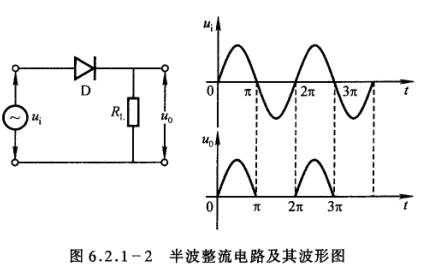
\includegraphics[width=0.7\linewidth]{img/1.png}
    \end{Figure}
    \subsubsection{全波整流}
    \begin{Figure}
        \centering
        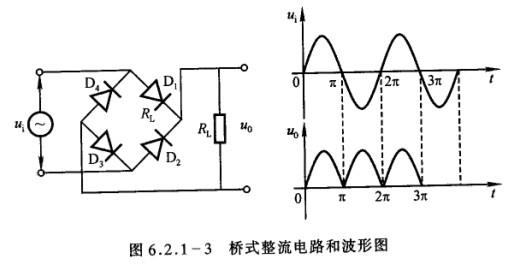
\includegraphics[width=0.7\linewidth]{img/2.png}
    \end{Figure}

    \subsubsection{电容滤波电路}

    在全波整流电路的基础上,添加一个电容$C$来作为反电动势。在电压上升时储能(降低电压峰值);在电压下降时充当蓄电池的作用,始终维持两侧电压不能突变。
    \begin{Figure}
        \centering
        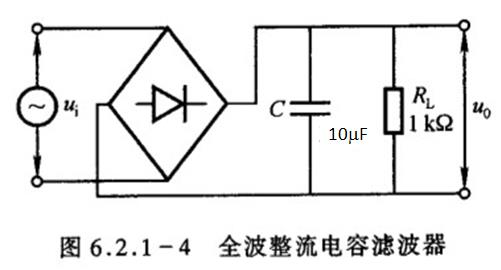
\includegraphics[width=0.7\linewidth]{img/3.png}
    \end{Figure}

    \subsubsection{\texorpdfstring{$\pi-RC$} -滤波}

    在上述方法的基础上,由于增大电容容量难以在实际应用中实现,于是利用以下电路了来进一步平滑输出电压:

    \begin{Figure}
        \centering
        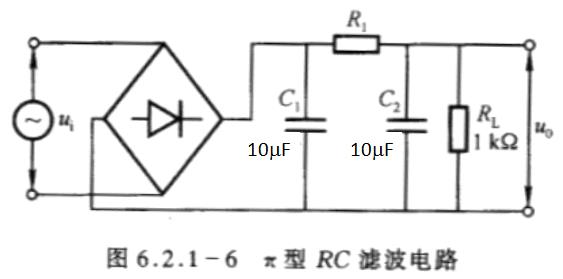
\includegraphics[width=0.7\linewidth]{img/4.png}
    \end{Figure}

    \subsection{纹波系数}

    纹波系数是用来评估整流滤波后电流的平滑度的, 纹波系数$K_u$越小,电流越平滑,表达式为:

    $$K_u = \dfrac{\bar U_{AC}}{\bar U_{DC}} \times 100 \%$$


    \section{实验方法}

    \subsection{整流、滤波实验}
    \begin{Figure}
        \centering
        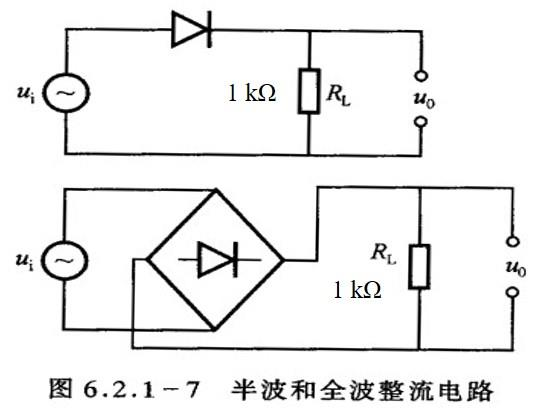
\includegraphics[width=0.7\linewidth]{img/5.png}
    \end{Figure}

    \begin{itemize}
        \item 按照上图构建电路,然后用示波器观测信号输出端的电压值(输入电压峰峰值$10V, f=400Hz$,分别观察初始信号、半波信号、全波信号的波形,并画出示意图。
        \item 在全波整流电路中,接入电容($C= 1\mu F$)进行滤波,用示波器观察输出端波形,同时用万用表测量直流、交流电压,计算纹波系数。
        \item 更换为$\pi-RC$电路后,观察波形,测量直流、交流电压,计算纹波系数。
    \end{itemize}

    \subsection{电容对滤波效果的影响}

    将电容更换为$C= 10\mu F$,重复上述(2)、(3)实验过程,对比波形差异和波纹系数,给出解释。

    \subsection{信号源频率对滤波效果的影响}

    固定电容$C= 1\mu F$,将信号源频率从$10Hz \sim 2000 Hz$(未必均匀变化),观察波形变化和纹波系数变化,同时比较两种滤波电路的差别。

    \subsection{探究影响整流滤波影响因素}

    在以上实验结果的基础上,替换电容为可调节的电容箱,固定电源$400Hz,U_{p-p} = 10 V$不变,调节电容大小($0.1\sim 1\mu F$),观察波形变化和直、交流成分的变化。综合分析以上影响因子对纹波系数的影响。

    \section{实验数据}

    \subsection{实验图像}
    在文章末尾会附上现场的照片,下面是经过处理后的数据:

    初始信号:
    \begin{Figure}
        \centering
        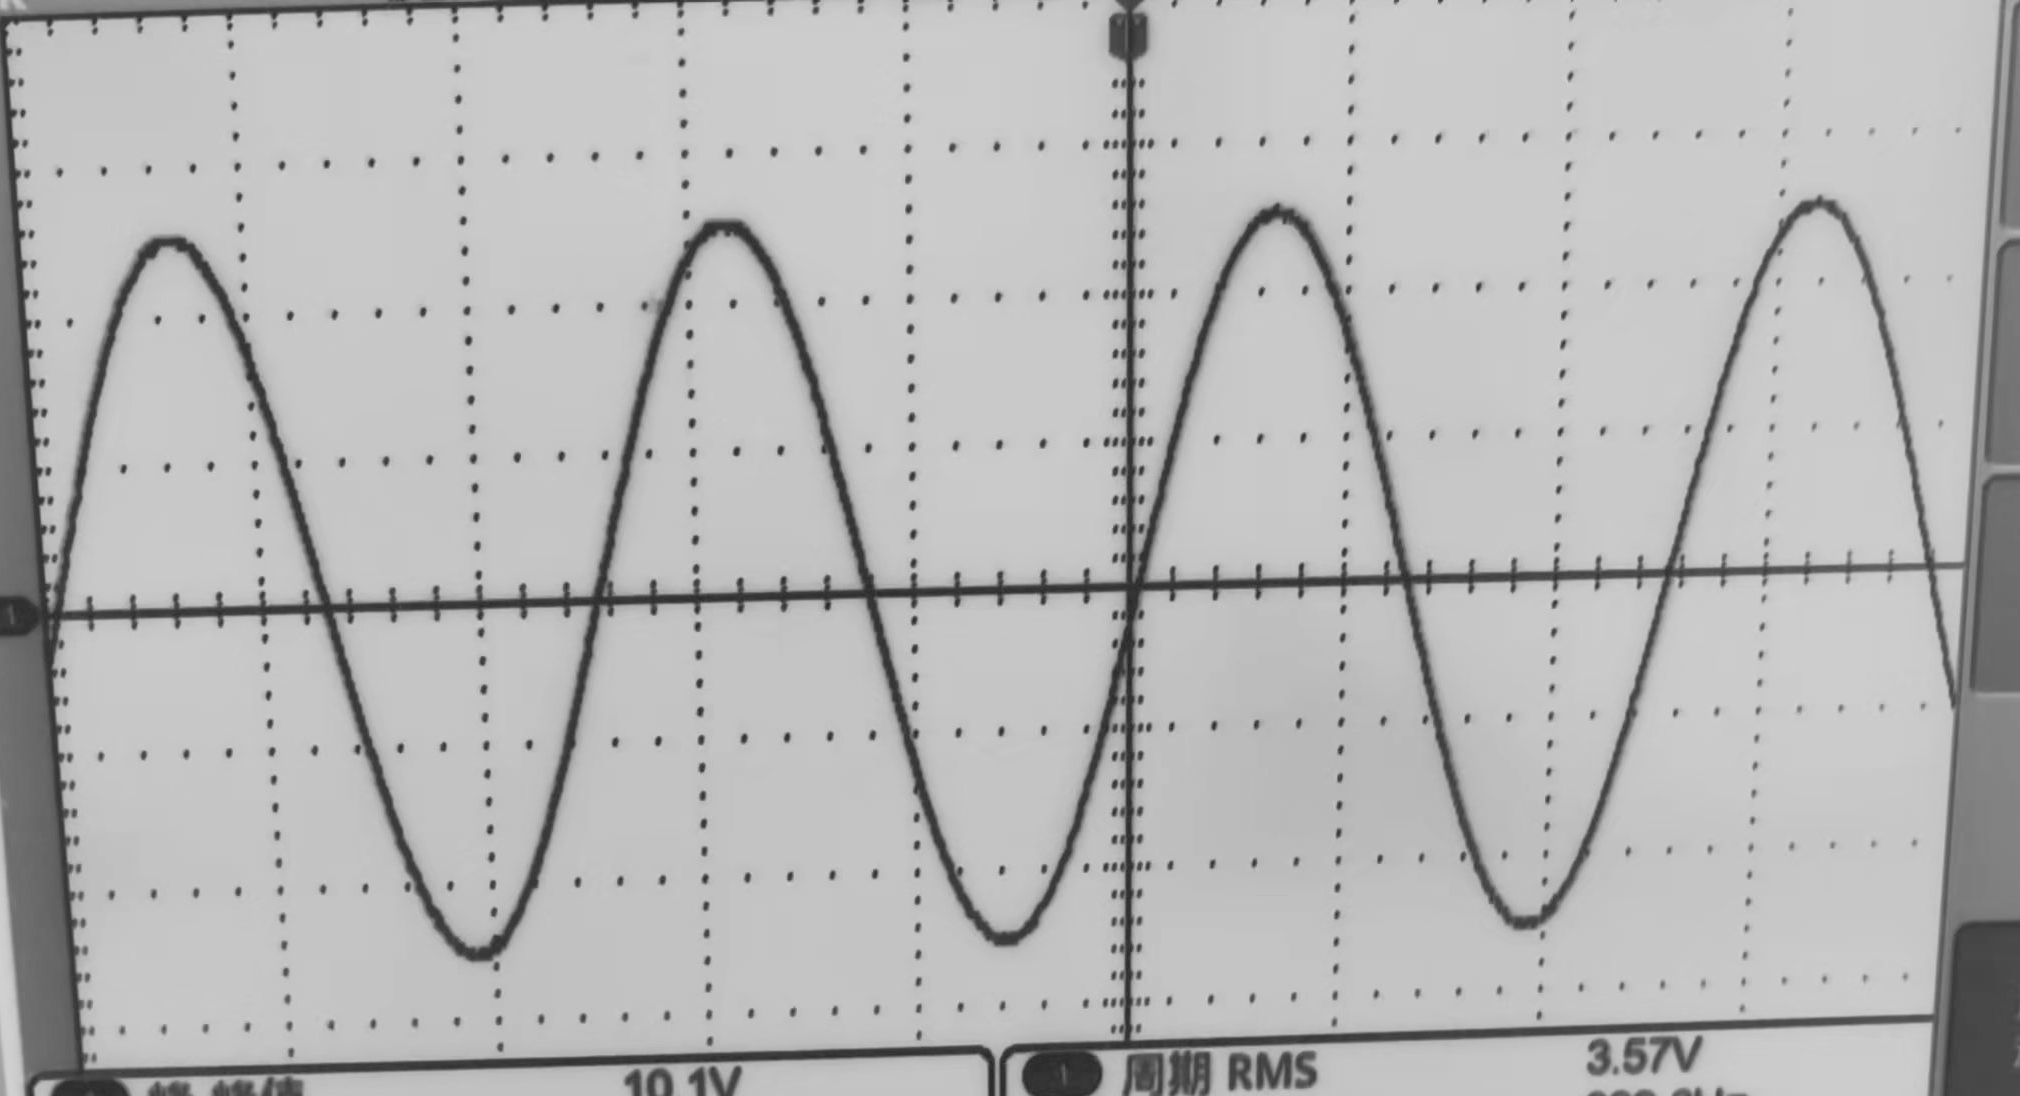
\includegraphics[width=0.7\linewidth]{img/done_edit/22.png}
    \end{Figure}

    半波信号:
    \begin{Figure}
        \centering
        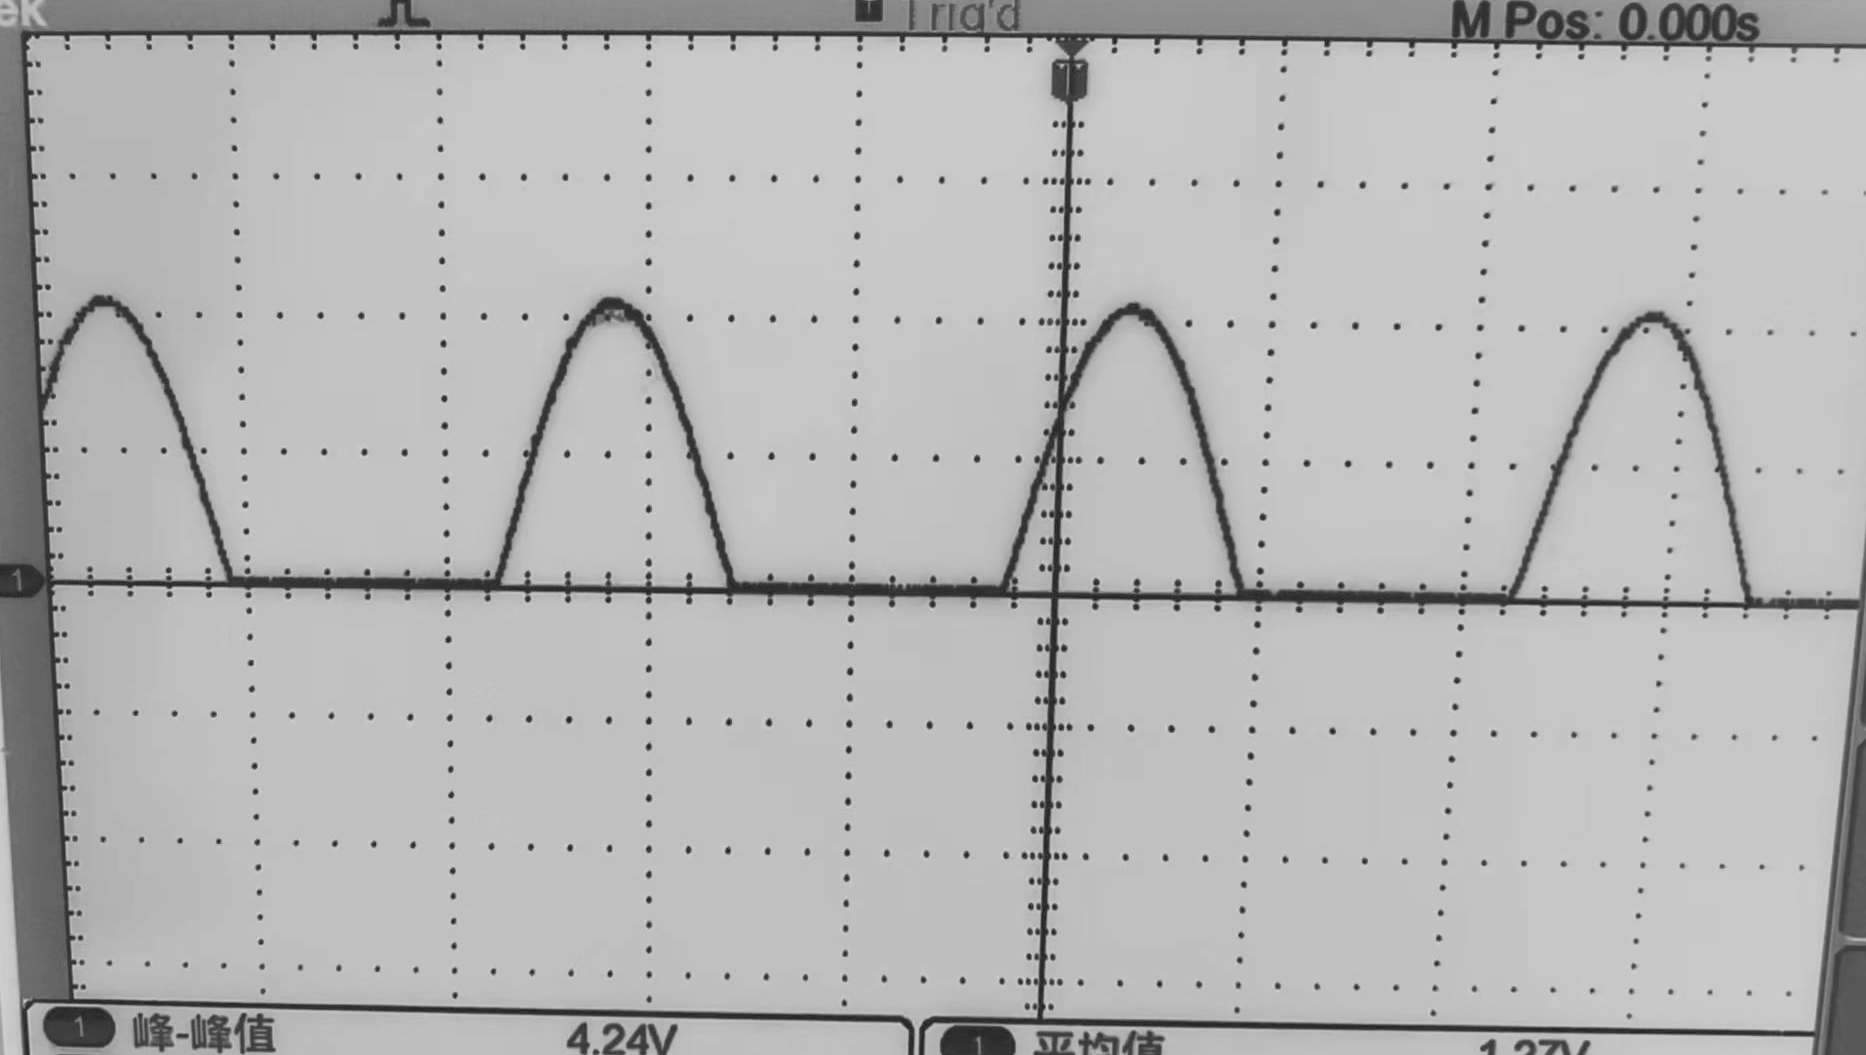
\includegraphics[width=0.7\linewidth]{img/done_edit/1.png}
    \end{Figure}

    全波信号:
    \begin{Figure}
        \centering
        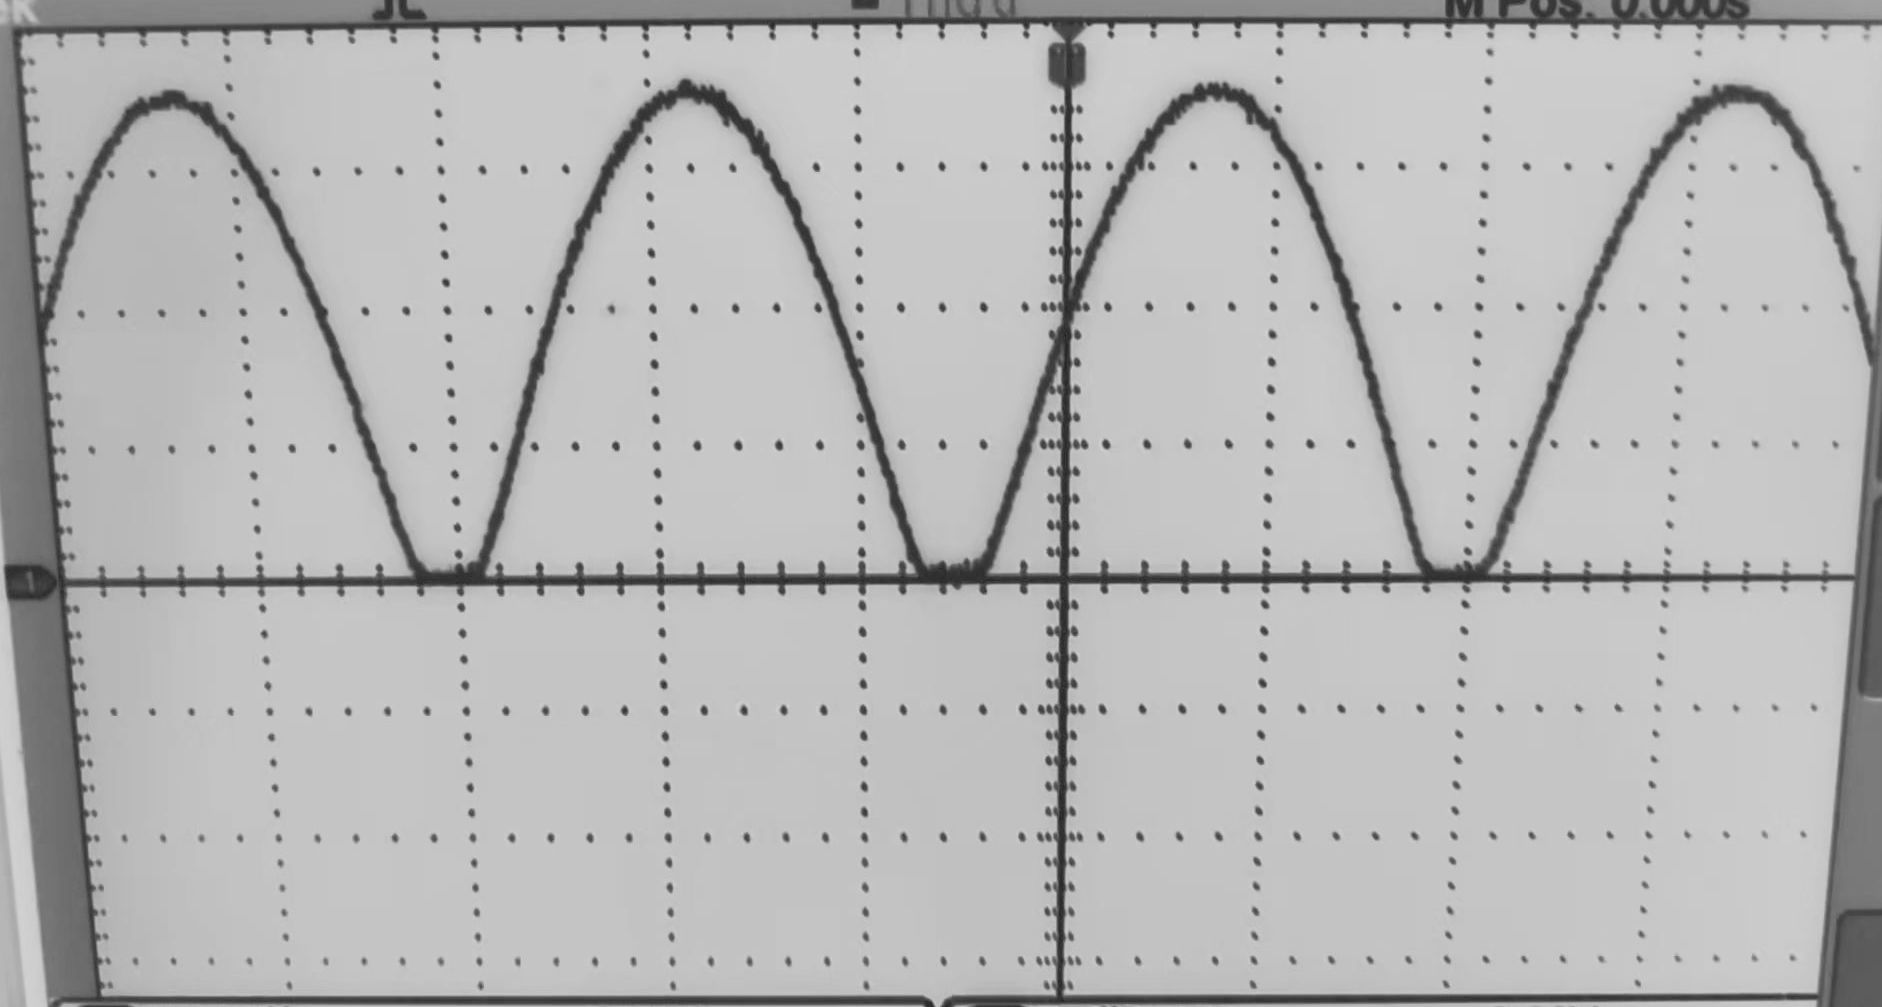
\includegraphics[width=0.7\linewidth]{img/done_edit/5.png}
    \end{Figure}

    $1\mu F$单电容滤波信号:
    \begin{Figure}
        \centering
        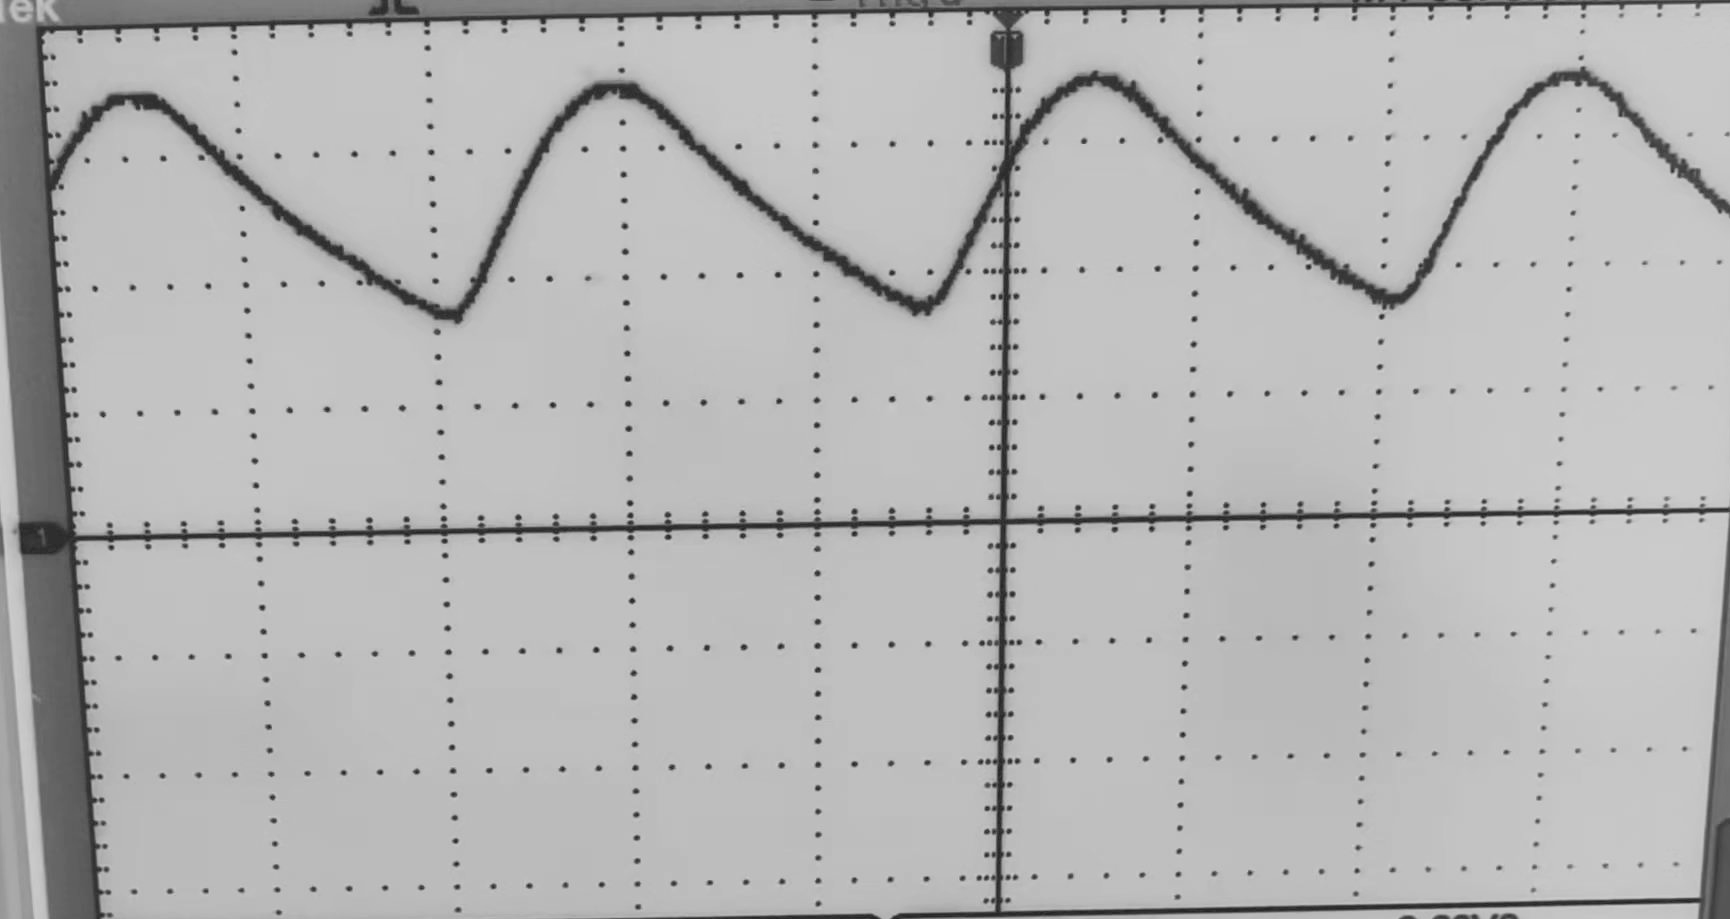
\includegraphics[width=0.7\linewidth]{img/done_edit/9.png}
    \end{Figure}

    $1\mu F$ $\pi - RC$滤波信号:
    \begin{Figure}
        \centering
        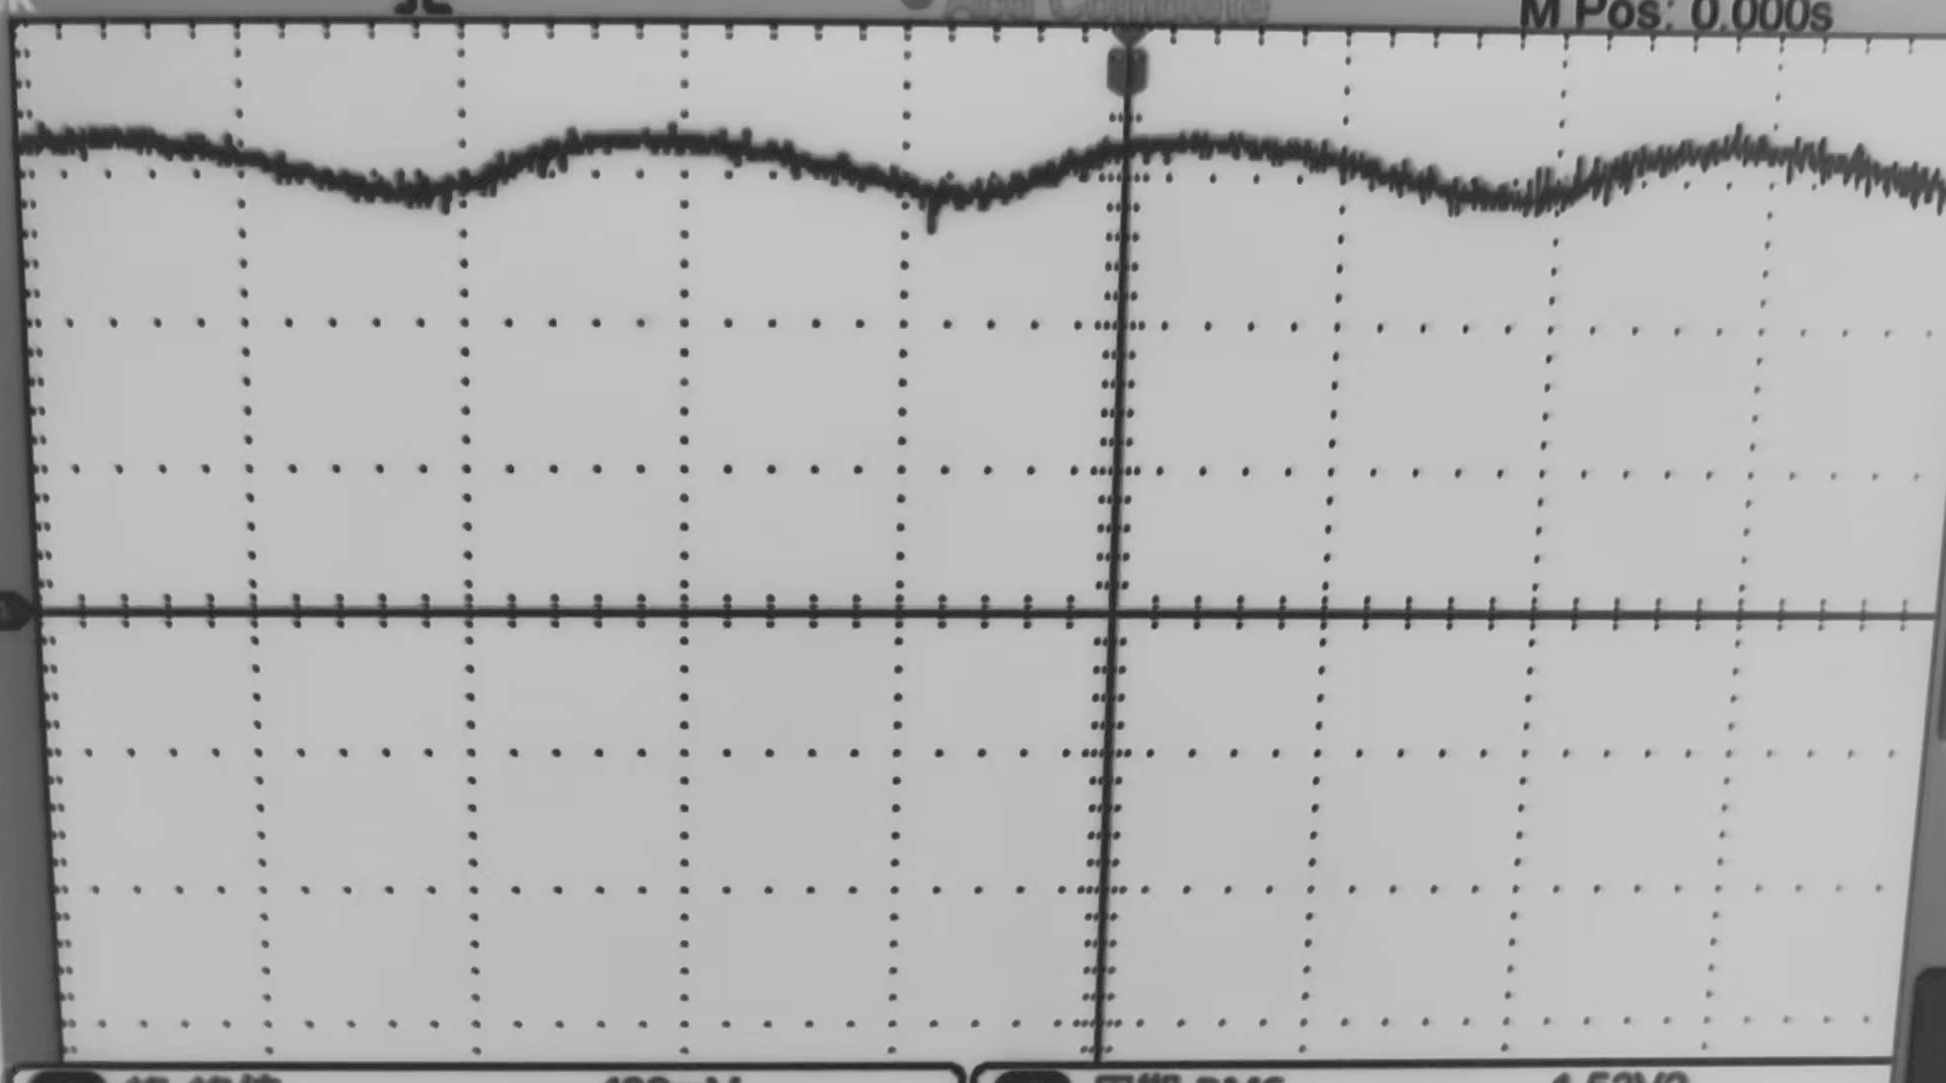
\includegraphics[width=0.7\linewidth]{img/done_edit/10.png}
    \end{Figure}

    $10\mu F$单电容滤波信号:
    \begin{Figure}
        \centering
        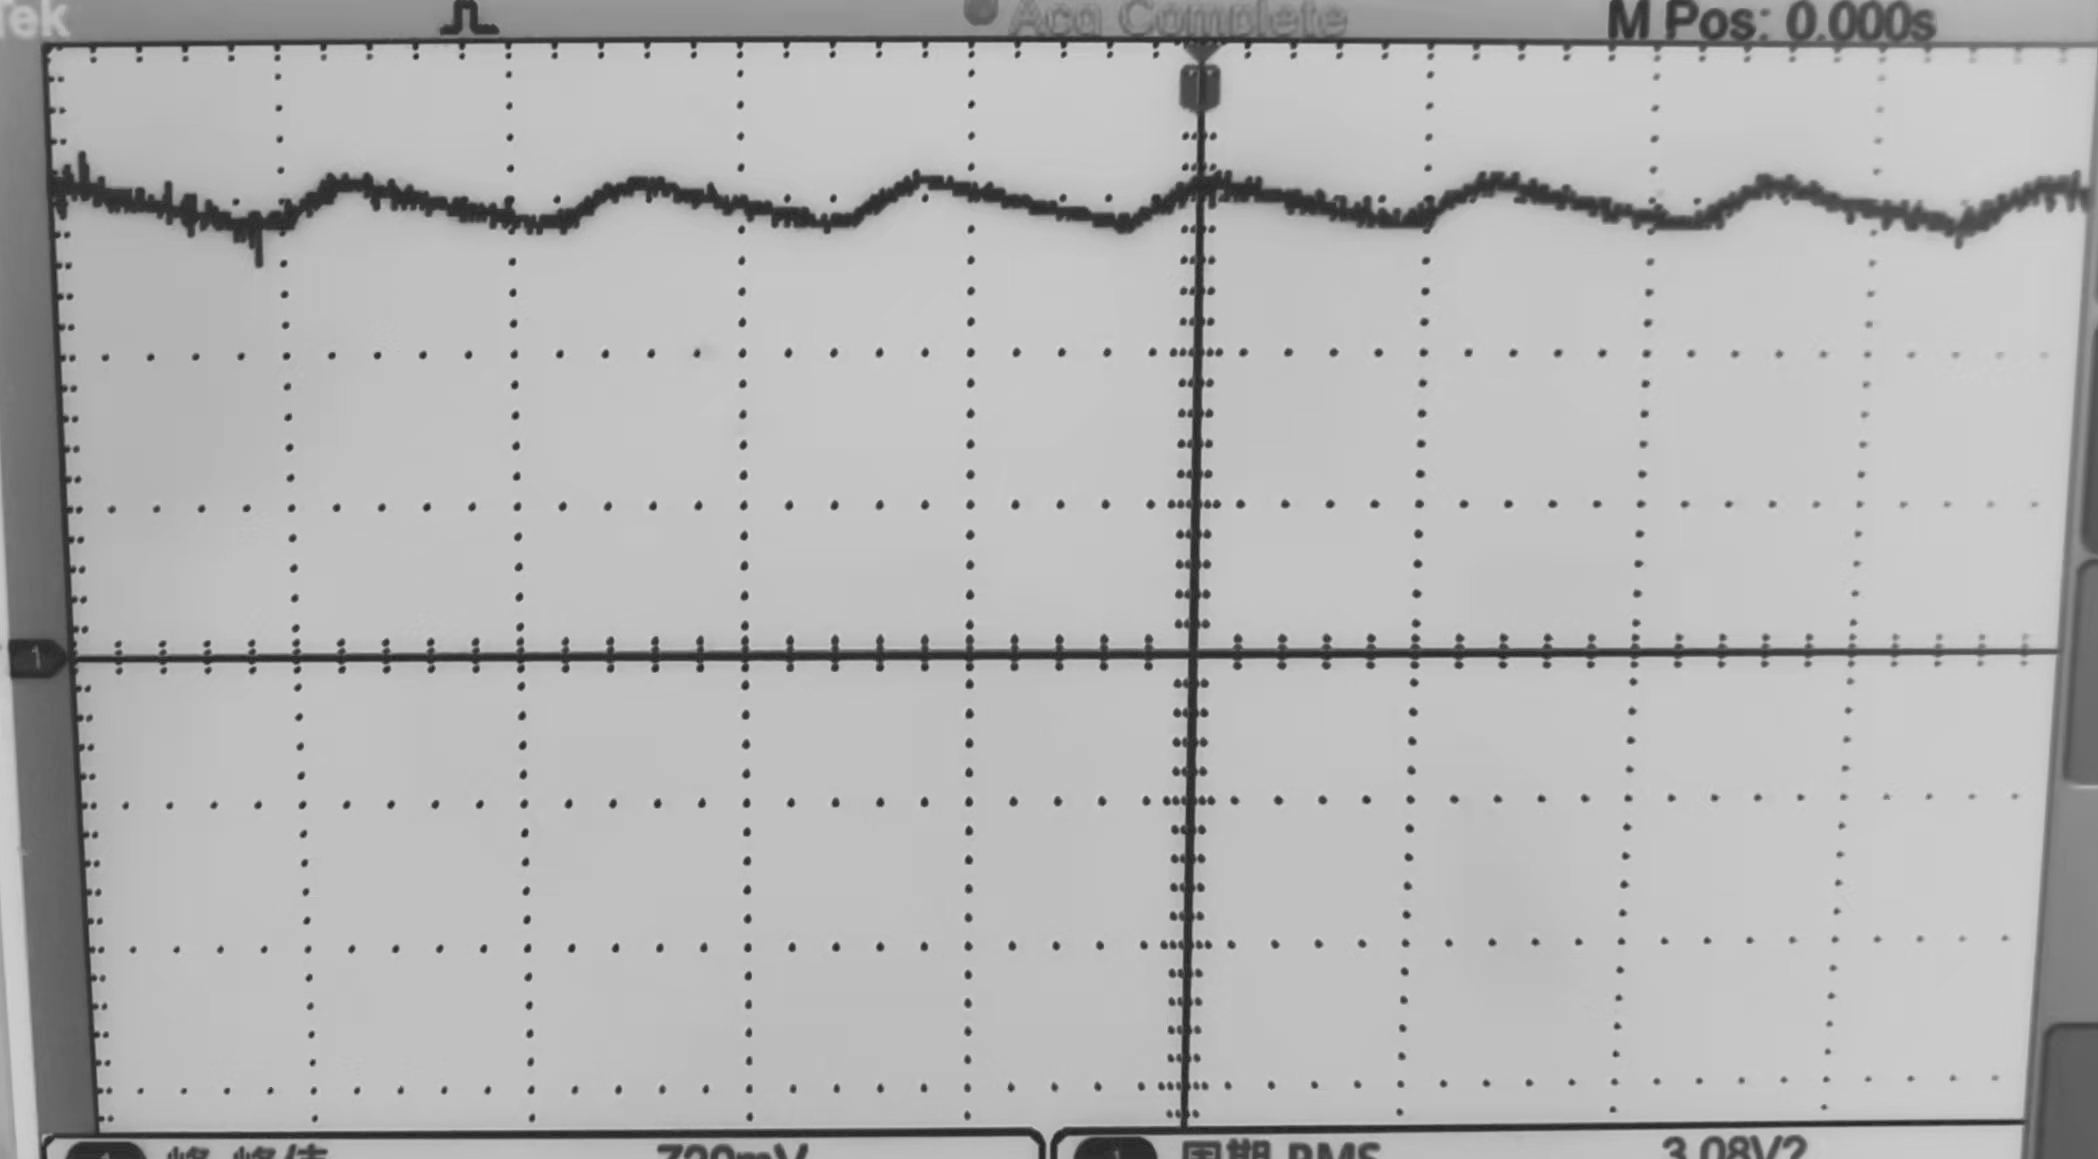
\includegraphics[width=0.7\linewidth]{img/done_edit/7.png}
    \end{Figure}

    $10\mu F$ $\pi - RC$滤波信号:
    \begin{Figure}
        \centering
        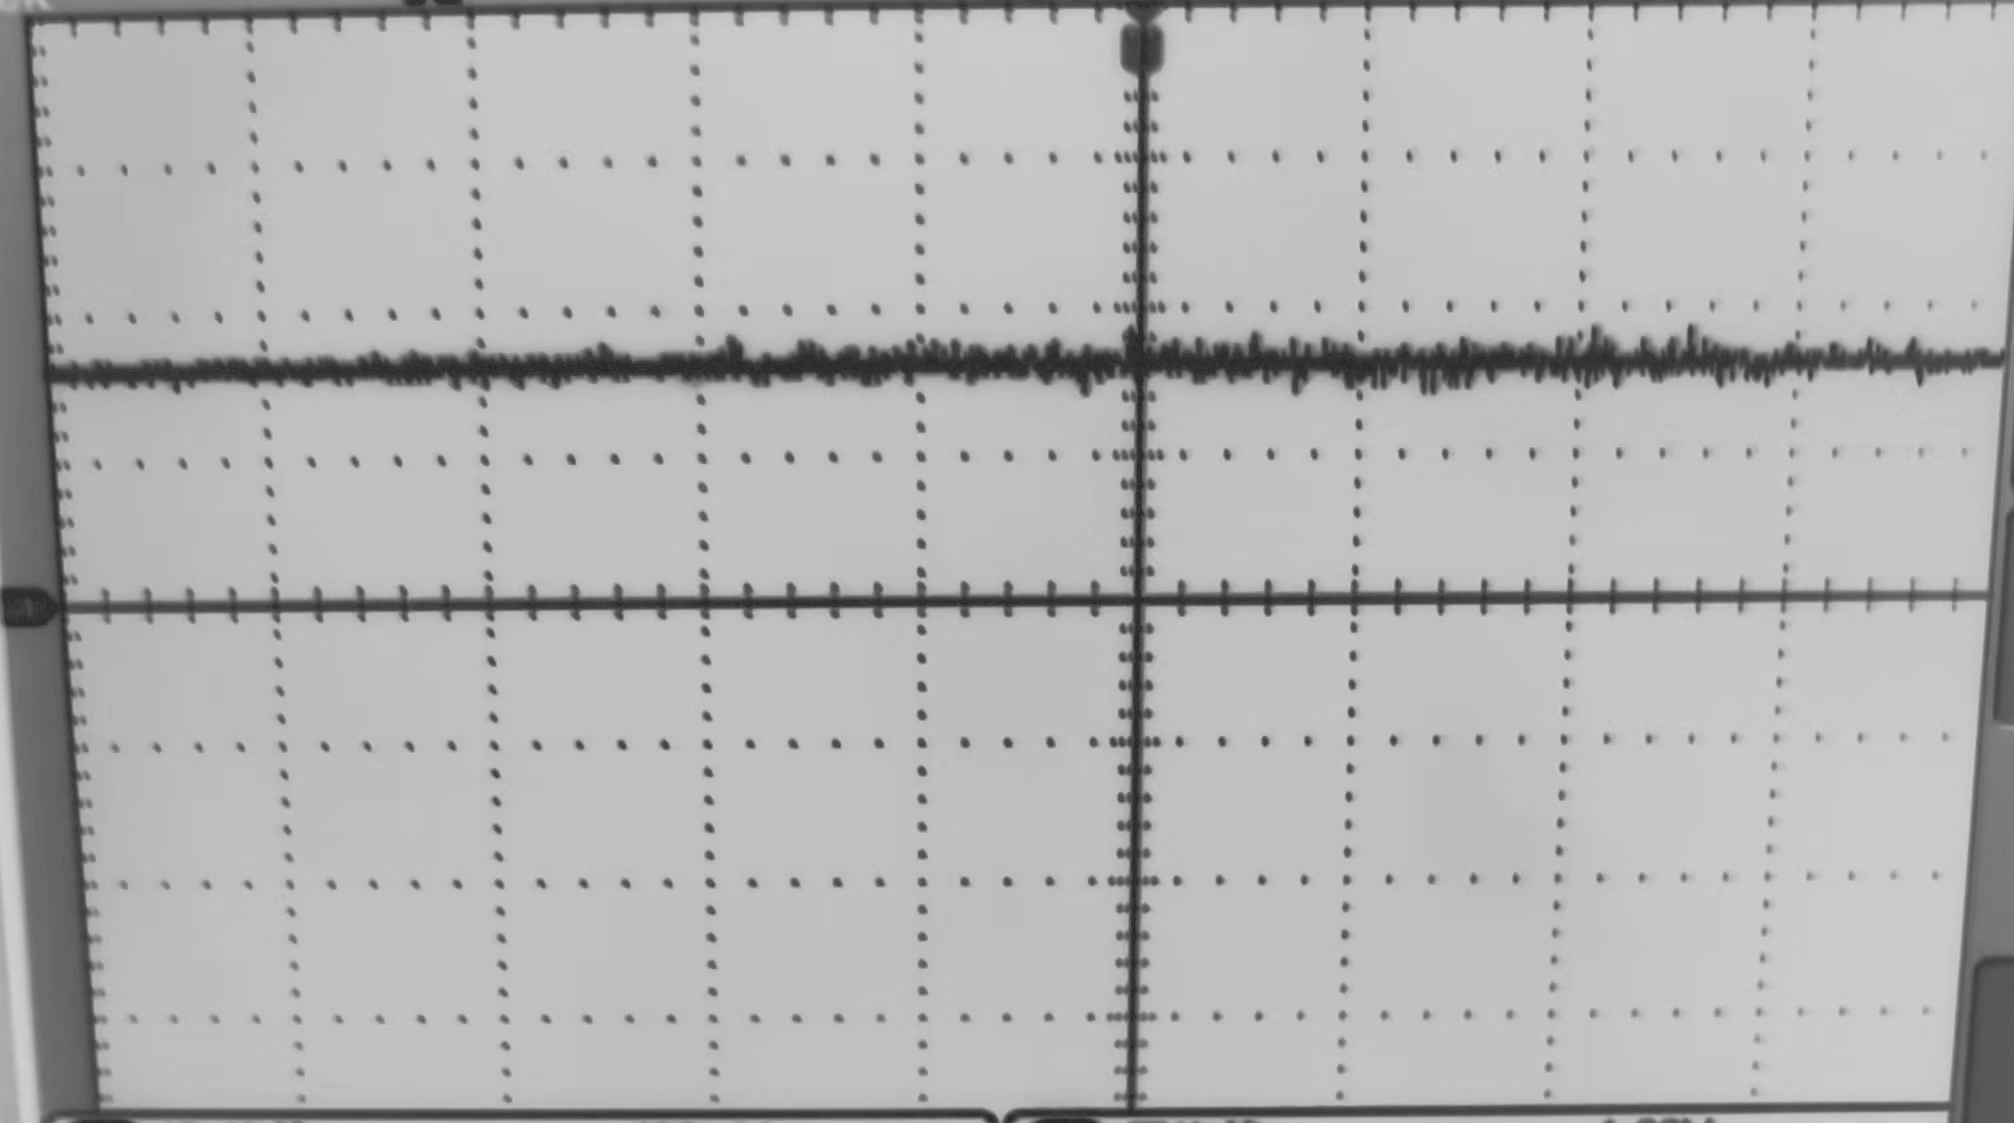
\includegraphics[width=0.7\linewidth]{img/done_edit/6.png}
    \end{Figure}

    \subsection{整流、滤波实验}
    $1\mu F$单电容滤波:$V_{DC} = 2.547 V, V_{AC} = 0.5711V$

    $1\mu F$ $\pi - RC$滤波:$V_{DC} = 1.4862 V, V_{AC} = 0.626V$
    \subsection{电容对滤波效果的影响}
    $10\mu F$单电容滤波:$V_{DC} = 2.908 V, V_{AC} = 0.0739V$

    $10\mu F$ $\pi - RC$滤波:$V_{DC} = 1.5715 V, V_{AC} <1mV$
\end{multicols}

\dotfill
\smallskip
\subsection{信号源频率对滤波效果的影响}
当$C=1\mu F, V_{P-P} = 10V$时:

\begin{tabular}{|c|c|c|c|c|}
    \hline \textbf{$f$} & \textbf{单电容滤波$V_{DC}$} & \textbf{~$V_{AC}$} & \textbf{$\pi - RC$滤波$V_{DC}$} & \textbf{~$V_{AC}$} \\
    \hline 10Hz         & 0.9963V                     & 0.6186V            & 1.8958V                         & 1.1987V            \\
    \hline 20Hz         & 1.045V                      & 0.5894V            & 1.9536V                         & 1.2360V            \\
    \hline 50Hz         & 1.1055V                     & 0.4813V            & 2.001V                          & 1.1735V            \\
    \hline 100Hz        & 1.2255V                     & 0.3210V            & 2.096V                          & 1.0410V            \\
    \hline 200Hz        & 1.3488V                     & 0.1613V            & 2.295V                          & 0.8310V            \\
    \hline 500Hz        & 1.4996V                     & 0.0427V            & 2.615V                          & 0.4887V            \\
    \hline 1000Hz       & 1.5497V                     & 0.0113V            & 2.792V                          & 0.2610V            \\
    \hline 2000Hz       & 1.5615V                     & <1mV               & 2.865V                          & 0.061V             \\\hline
\end{tabular}

\subsection{探究影响整流滤波影响因素}
当$f=400Hz,V_{P-P}=10V$

\begin{multicols}{2}
    \begin{tabular}{|c|c|c|}
        \hline \textbf{C} & \textbf{$V_{DC}$} & \textbf{$V_{AC}$} \\
        \hline $1\mu F$   & 1.9721V           & 1.1827V           \\
        \hline $2\mu F$   & 2.050V            & 1.0880V           \\
        \hline $3\mu F$   & 2.138V            & 0.9923V           \\
        \hline $4\mu F$   & 2.220V            & 0.9048V           \\
        \hline $5\mu F$   & 2.298V            & 0.8279V           \\
        \hline $6\mu F$   & 2.368V            & 0.7614V           \\
        \hline $7\mu F$   & 2.429V            & 0.7030V           \\
        \hline $8\mu F$   & 2.476V            & 0.6494V           \\
        \hline $9\mu F$   & 2.522V            & 0.6047V           \\
        \hline $10\mu F$  & 2.562V            & 0.5649V           \\\hline
    \end{tabular}

    \section{实验结果}
    \subsection{整流、滤波实验}
    $1\mu F$单电容滤波:$K_U = 0.224$,

    $\pi- RC$滤波:$K_U = 0.421$

    \subsection{电容对滤波效果的影响}
    $10\mu F$单电容滤波:$K_U = 0.025$,

    $\pi- RC$滤波:$K_U<0.6\times 10^{-3}$

    \subsection{信号源频率对滤波效果的影响}
    \noindent
    $C = 1\mu F$时,$V_{DC},V_{AC} \sim f$的图像:

    其中$K_1$为单电容的情况,$K_2$为$\pi -RC$的情况($f$轴已取对数):
    \begin{Figure}
        \centering
        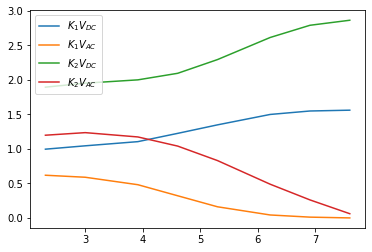
\includegraphics[width=0.8\linewidth]{img/6.png}
    \end{Figure}

    \noindent
    同时对比$K_u$系数:
    \begin{Figure}
        \centering
        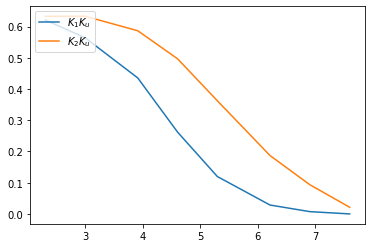
\includegraphics[width=0.8\linewidth]{img/7.png}
    \end{Figure}

    \noindent
    可以看出
    \begin{itemize}
        \item 随着$f$的逐渐增加,$V_{DC}$增加,$V_{AC}$减小,$K_u$减小。
        \item 使用$\pi -RC$滤波得到的直流电压始终比单电容的输出要高
        \item 单电容的$K_u$始终比使用$\pi-RC$的$K_u$要低。
    \end{itemize}

    \subsection{探究影响整流滤波影响因素}
    \noindent
    $f = 400 Hz$时,$V_{DC},V_{AC} \sim C$的图像:

    \begin{Figure}
        \centering
        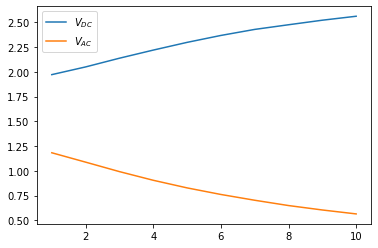
\includegraphics[width=0.8\linewidth]{img/8.png}
    \end{Figure}

    \noindent
    $K_u \sim C$的图像:

    \begin{Figure}
        \centering
        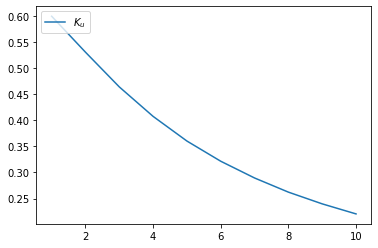
\includegraphics[width=0.8\linewidth]{img/9.png}
    \end{Figure}

    $K_u(C)$的拟合结果为:$K_u = 0.58 \times e^{-0.17 C} + 0.11$
    \begin{Figure}
        \centering
        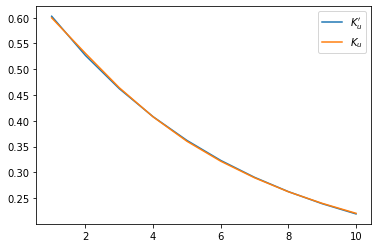
\includegraphics[width=0.8\linewidth]{img/10.png}
    \end{Figure}

    \subsection{结论}

    在实验测定的范围内,$K_u$和$f,C$的关系是:随着$f$的增大而减小,随着$C$的增大而减小,并未测得明显方程表示。

    \section{思考题}
    \begin{itemize}
        \item 整流、滤波的主要目的是什么?

              整流主要将交流电转为直流电,在一些交流电不可用的场景(比如电镀、锂电池充电等)。滤波的目的是平滑电流,更大限度地减小损耗。

        \item 滤波电路中电容是否越大越好?请根据实验过程简述理由。

              我的理解是,在一定范围内(例如实验测得的范围),电容越大,滤波效果越好,且输出电压更高。但随着电容增大,提高电容带来的效果收益会越来越小,出于成本考虑应该选用适中的电容。
    \end{itemize}
    \section{原始图像}

    初始信号:
    \begin{Figure}
        \centering
        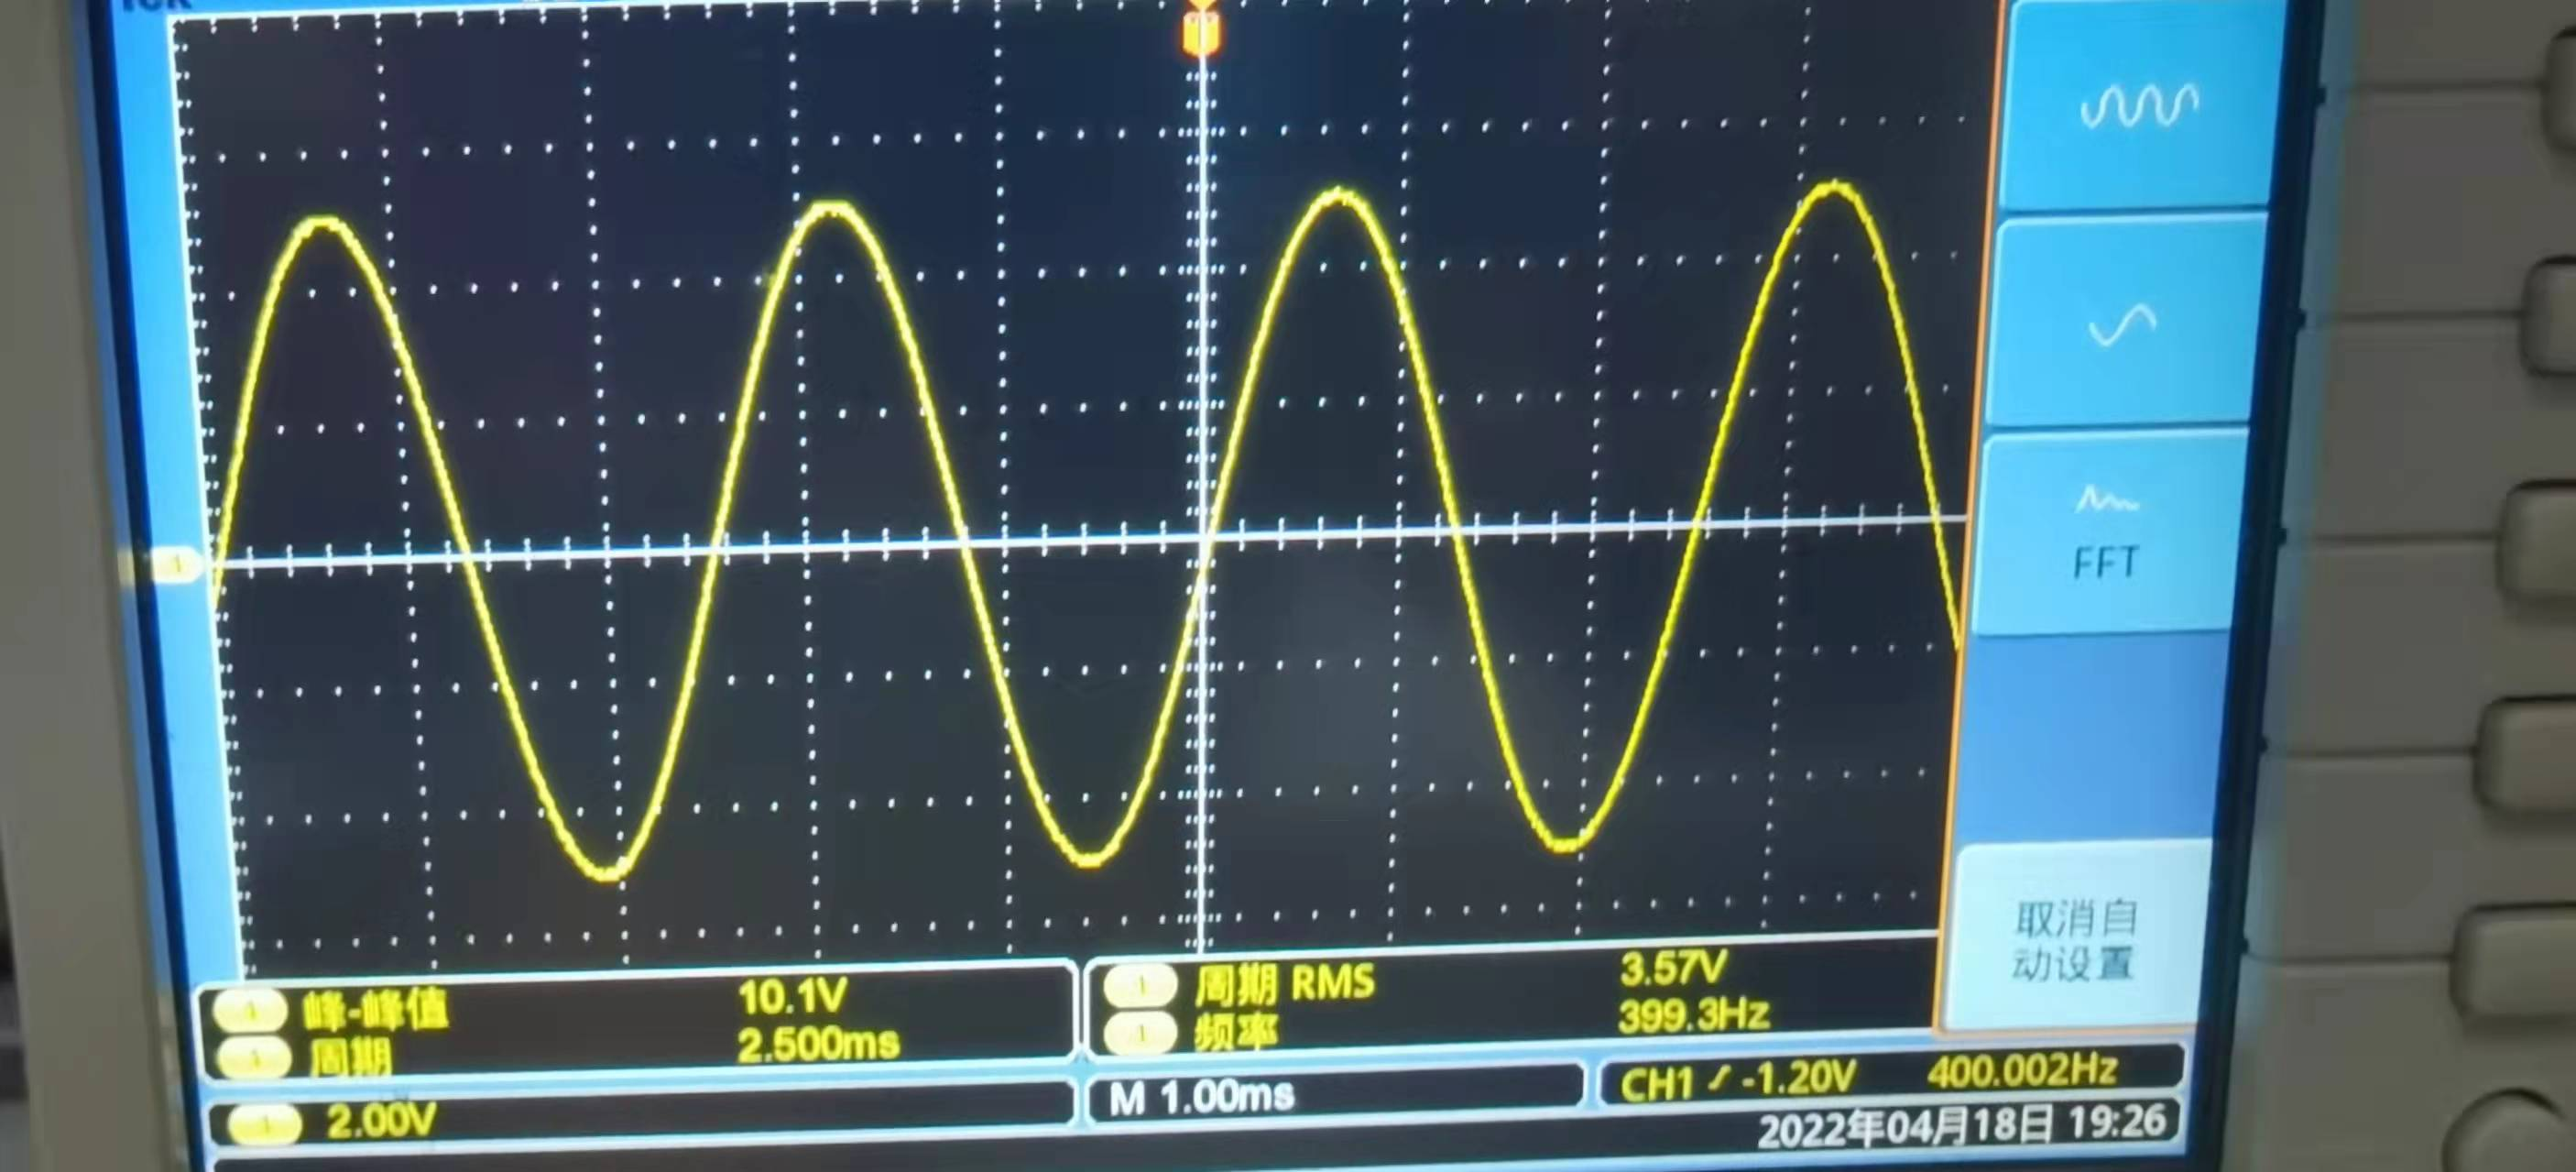
\includegraphics[width=0.7\linewidth]{img/original/22.jpg}
    \end{Figure}

    半波信号:
    \begin{Figure}
        \centering
        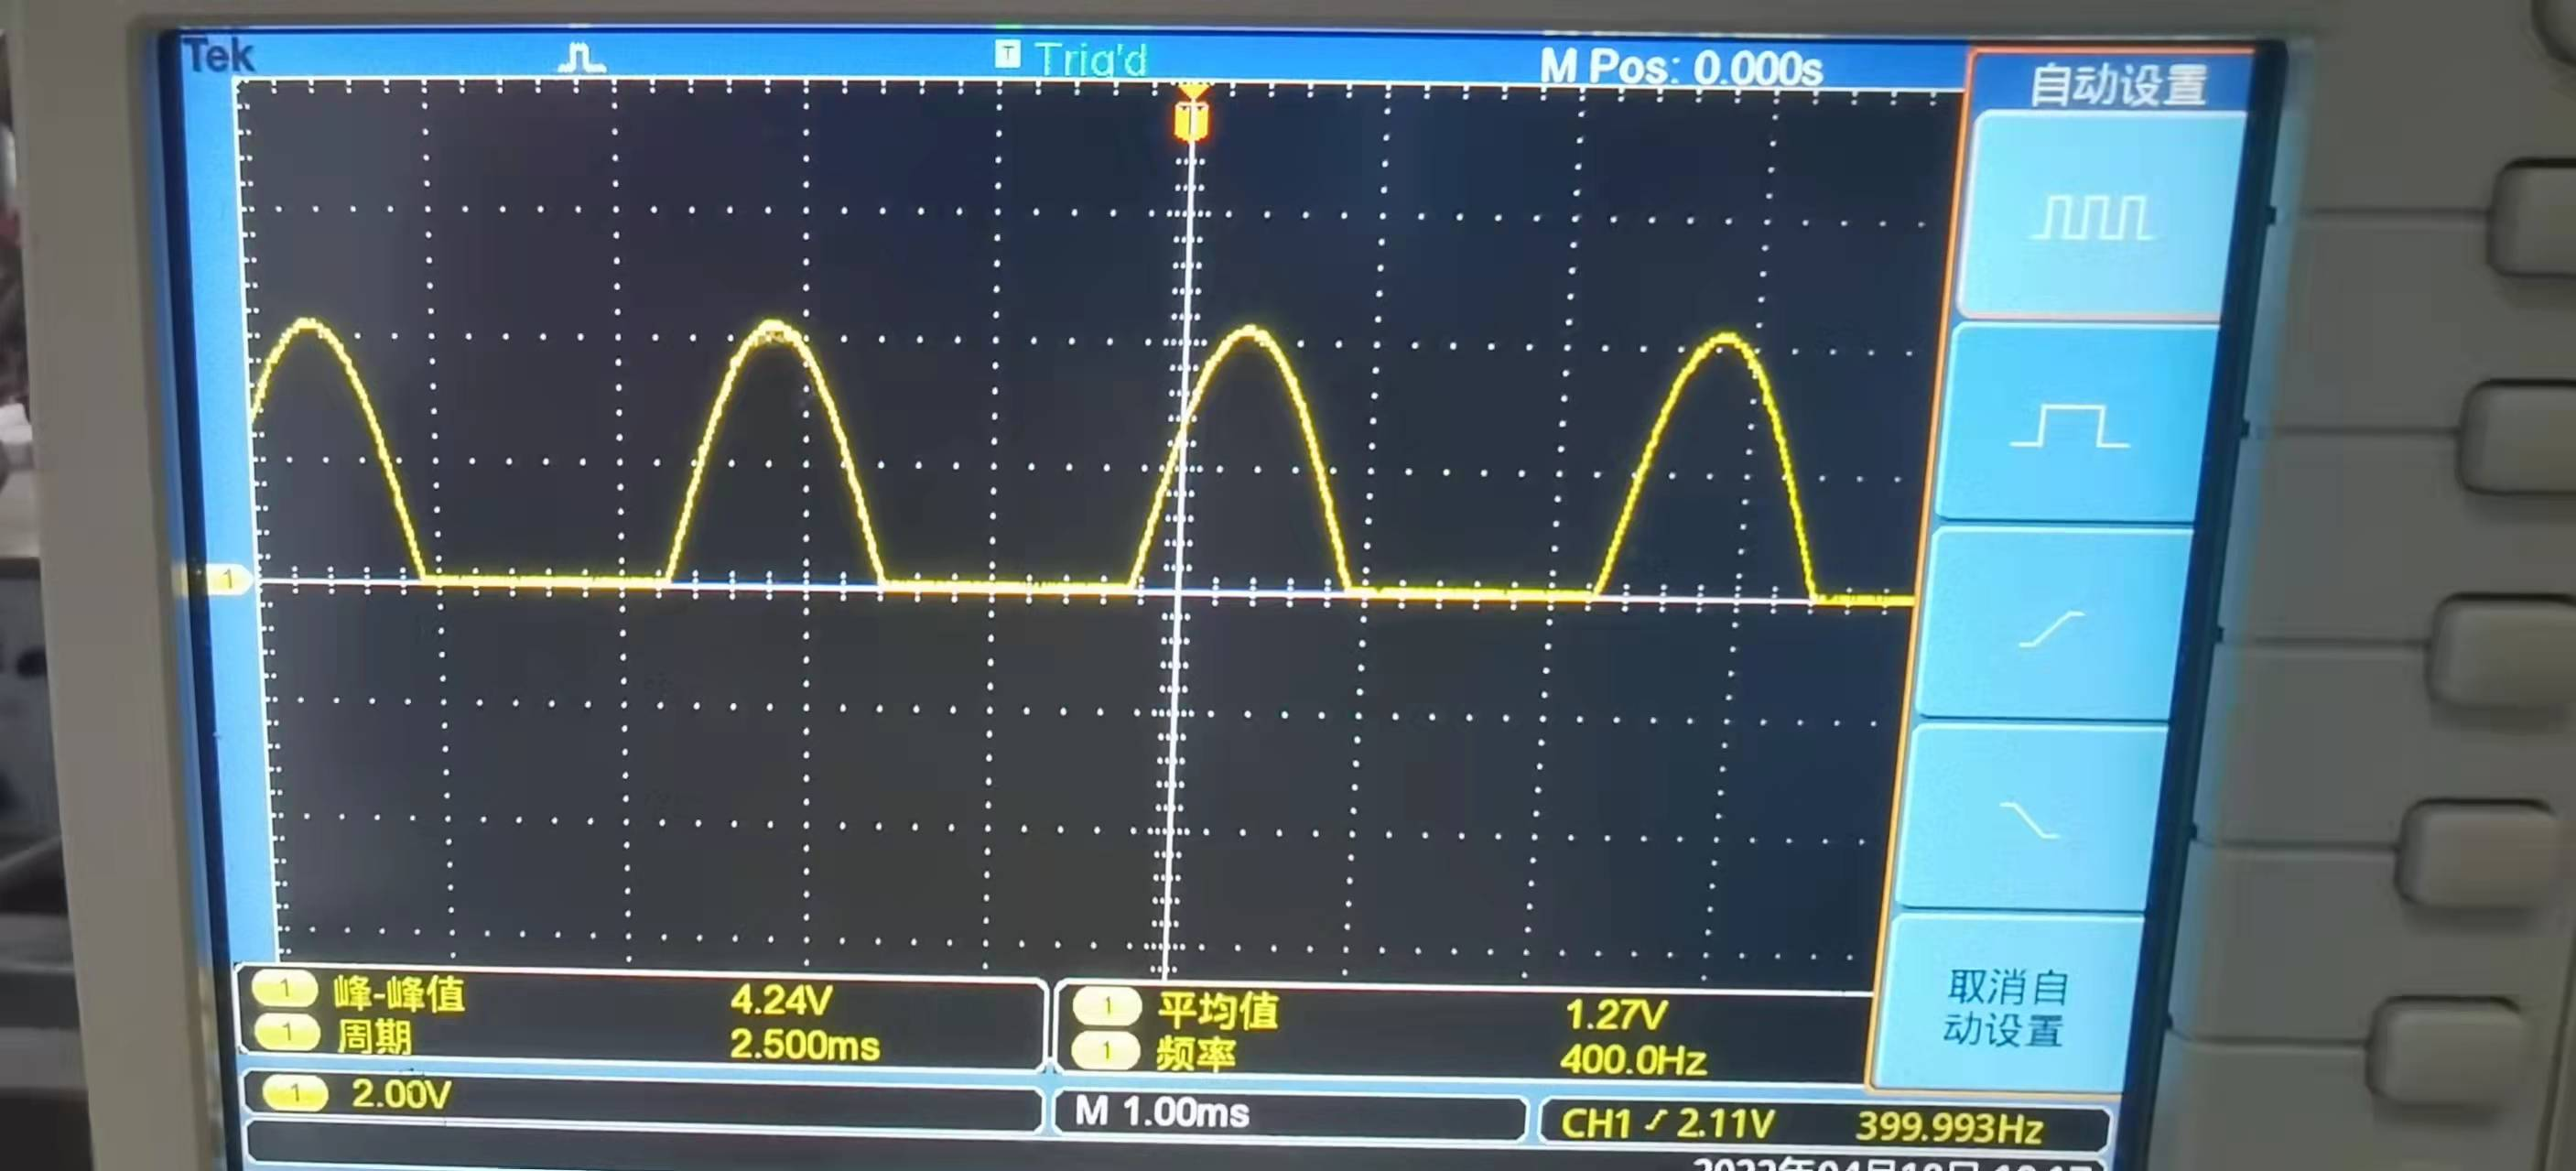
\includegraphics[width=0.7\linewidth]{img/original/1.jpg}
    \end{Figure}

    全波信号:
    \begin{Figure}
        \centering
        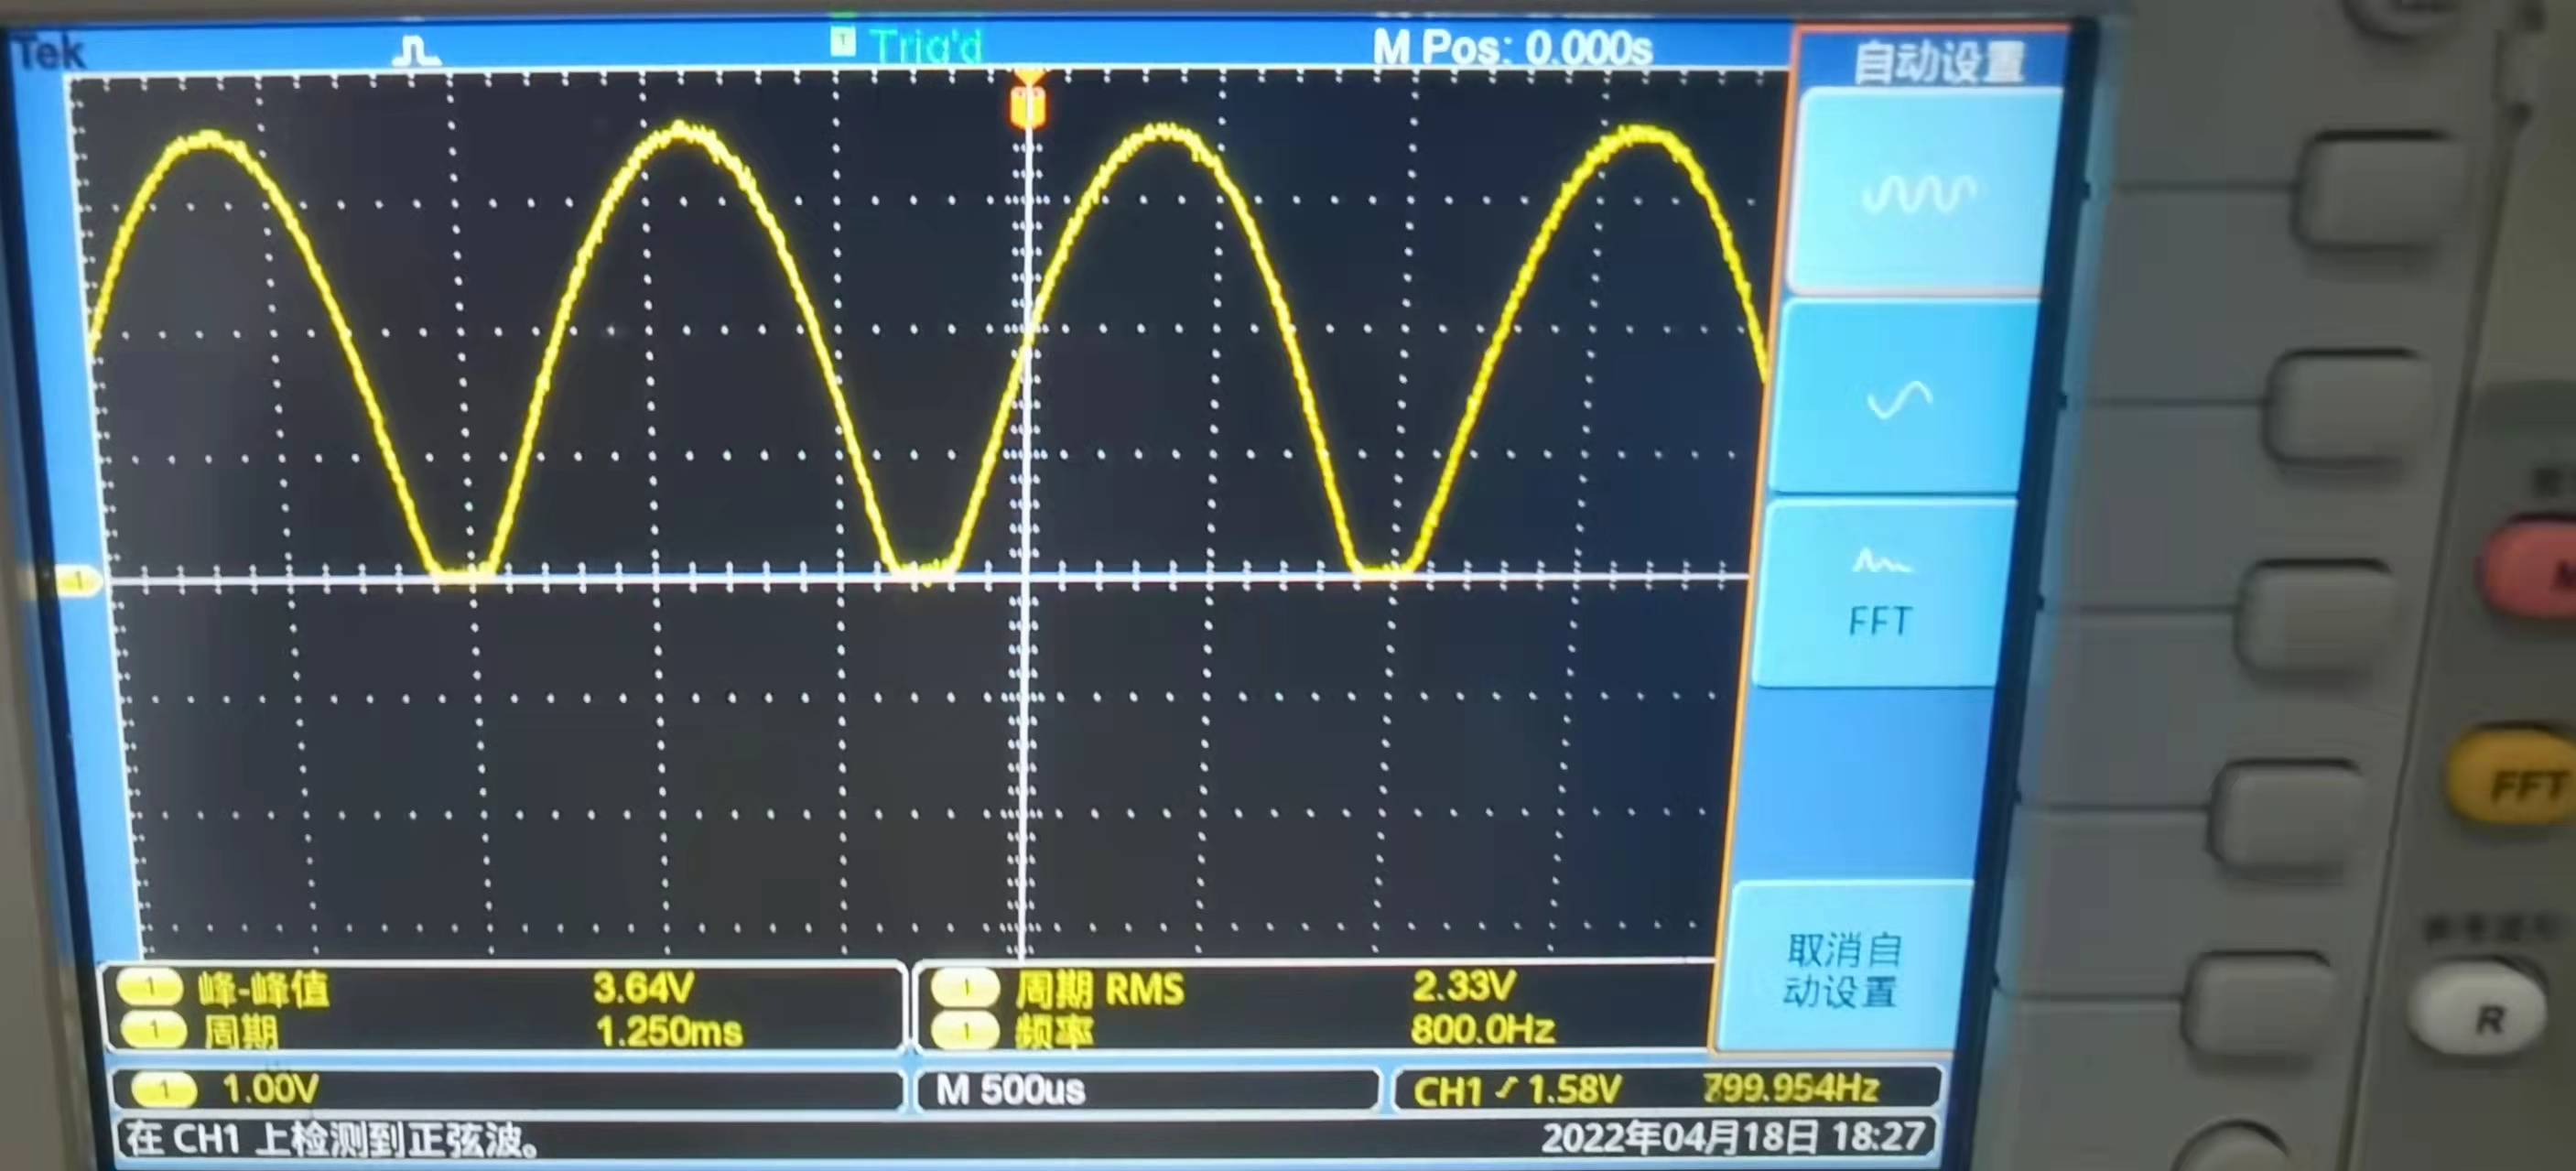
\includegraphics[width=0.7\linewidth]{img/original/5.jpg}
    \end{Figure}

    $1\mu F$单电容滤波信号:
    \begin{Figure}
        \centering
        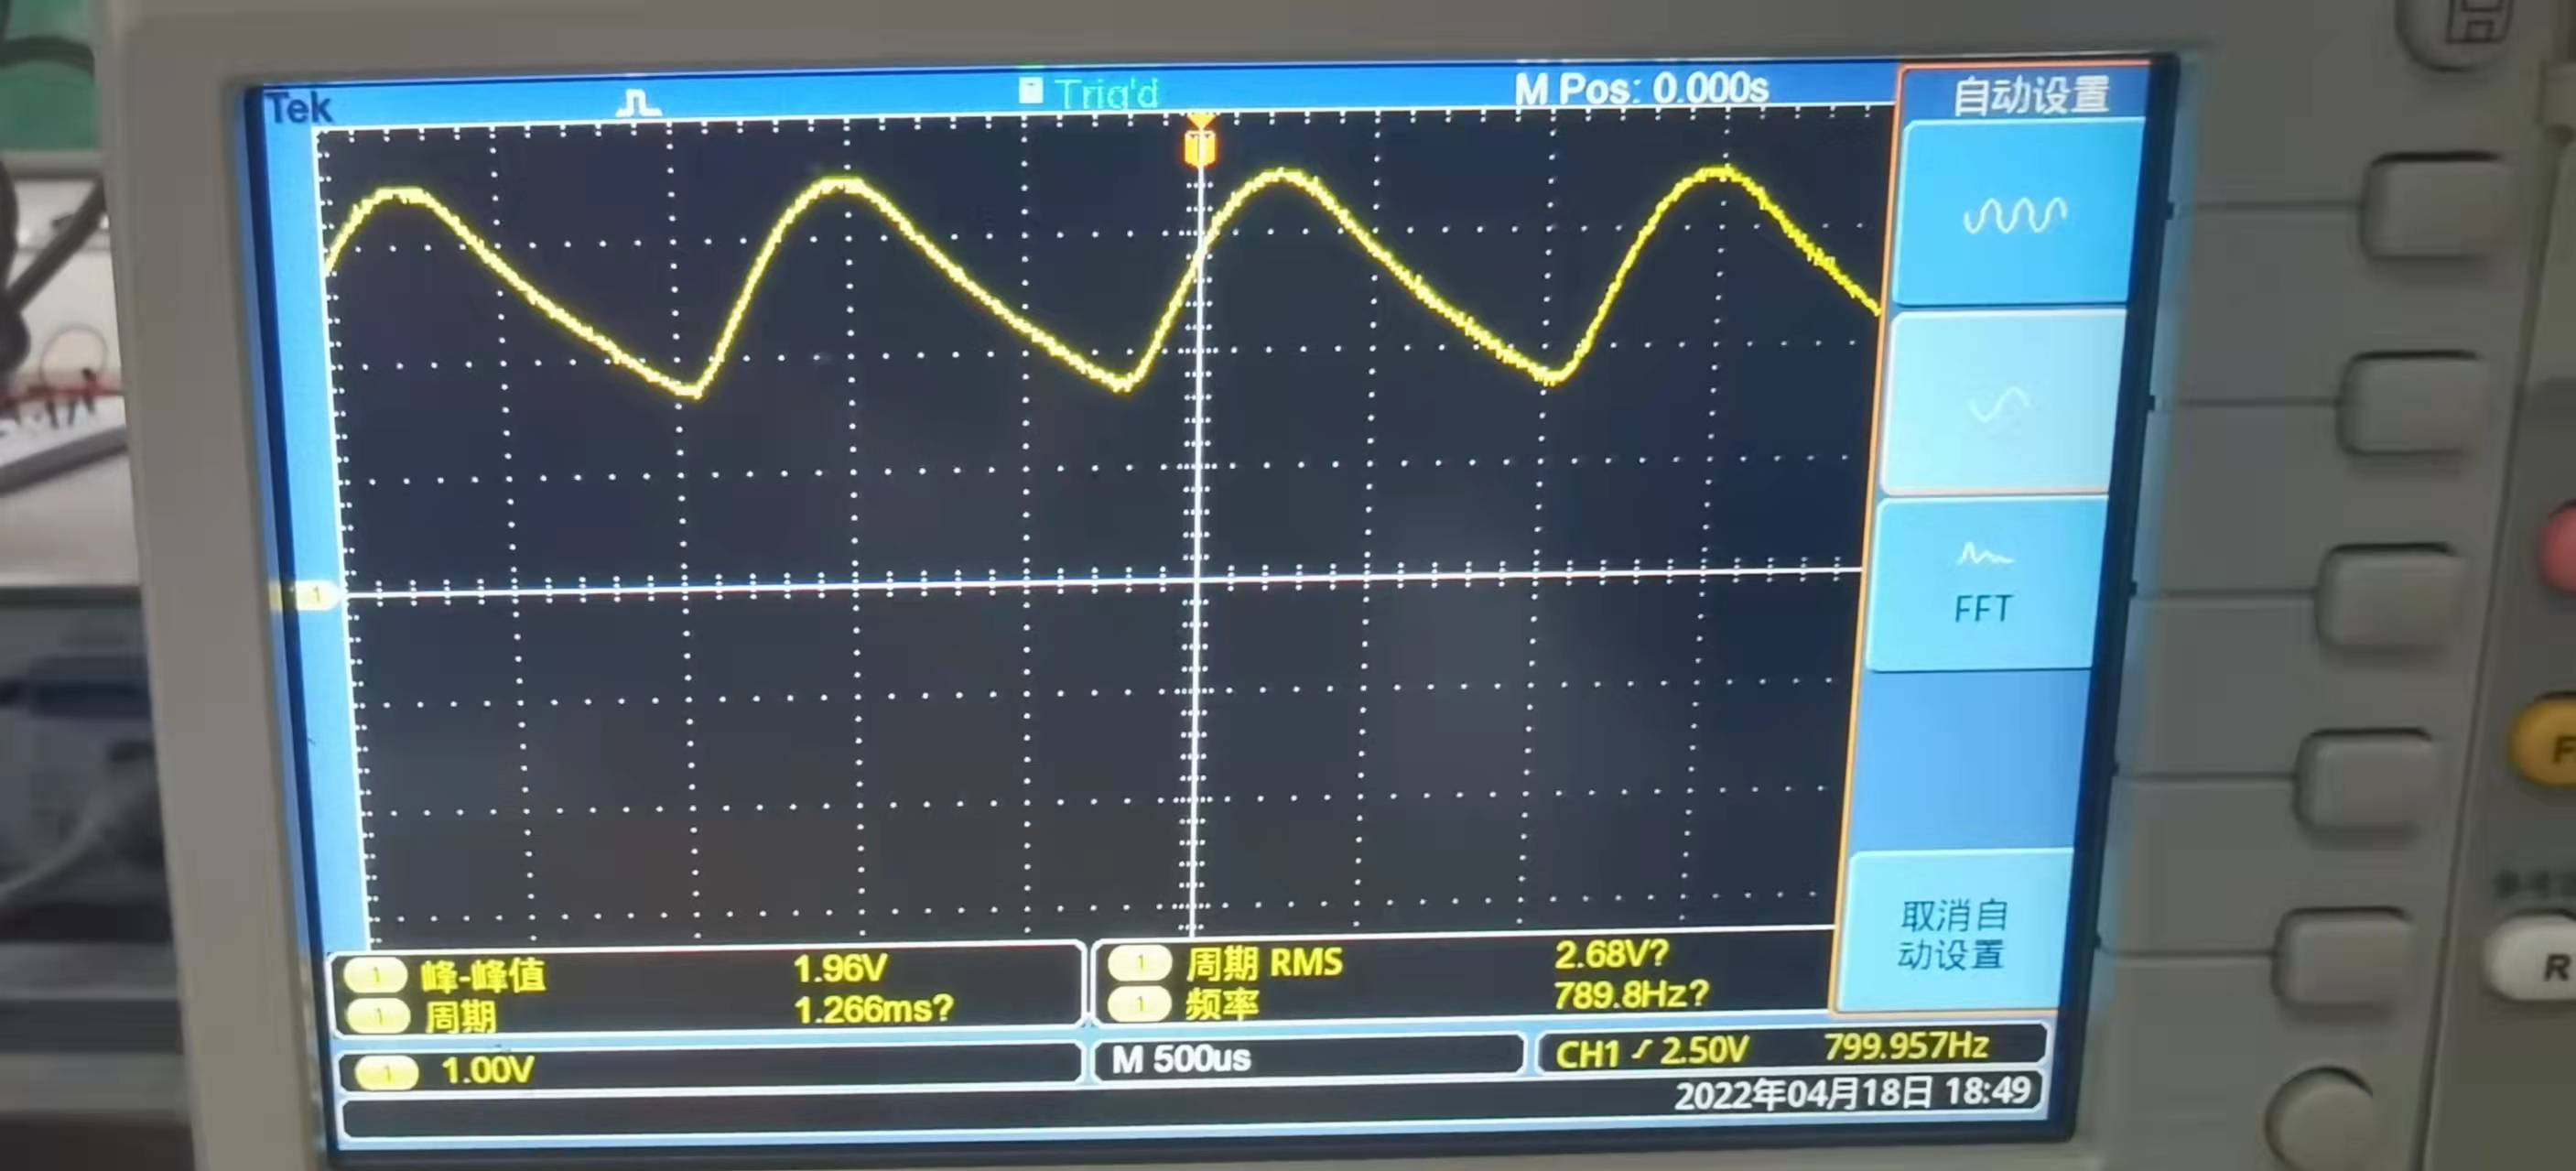
\includegraphics[width=0.7\linewidth]{img/original/9.jpg}
    \end{Figure}

    $1\mu F$ $\pi - RC$滤波信号:
    \begin{Figure}
        \centering
        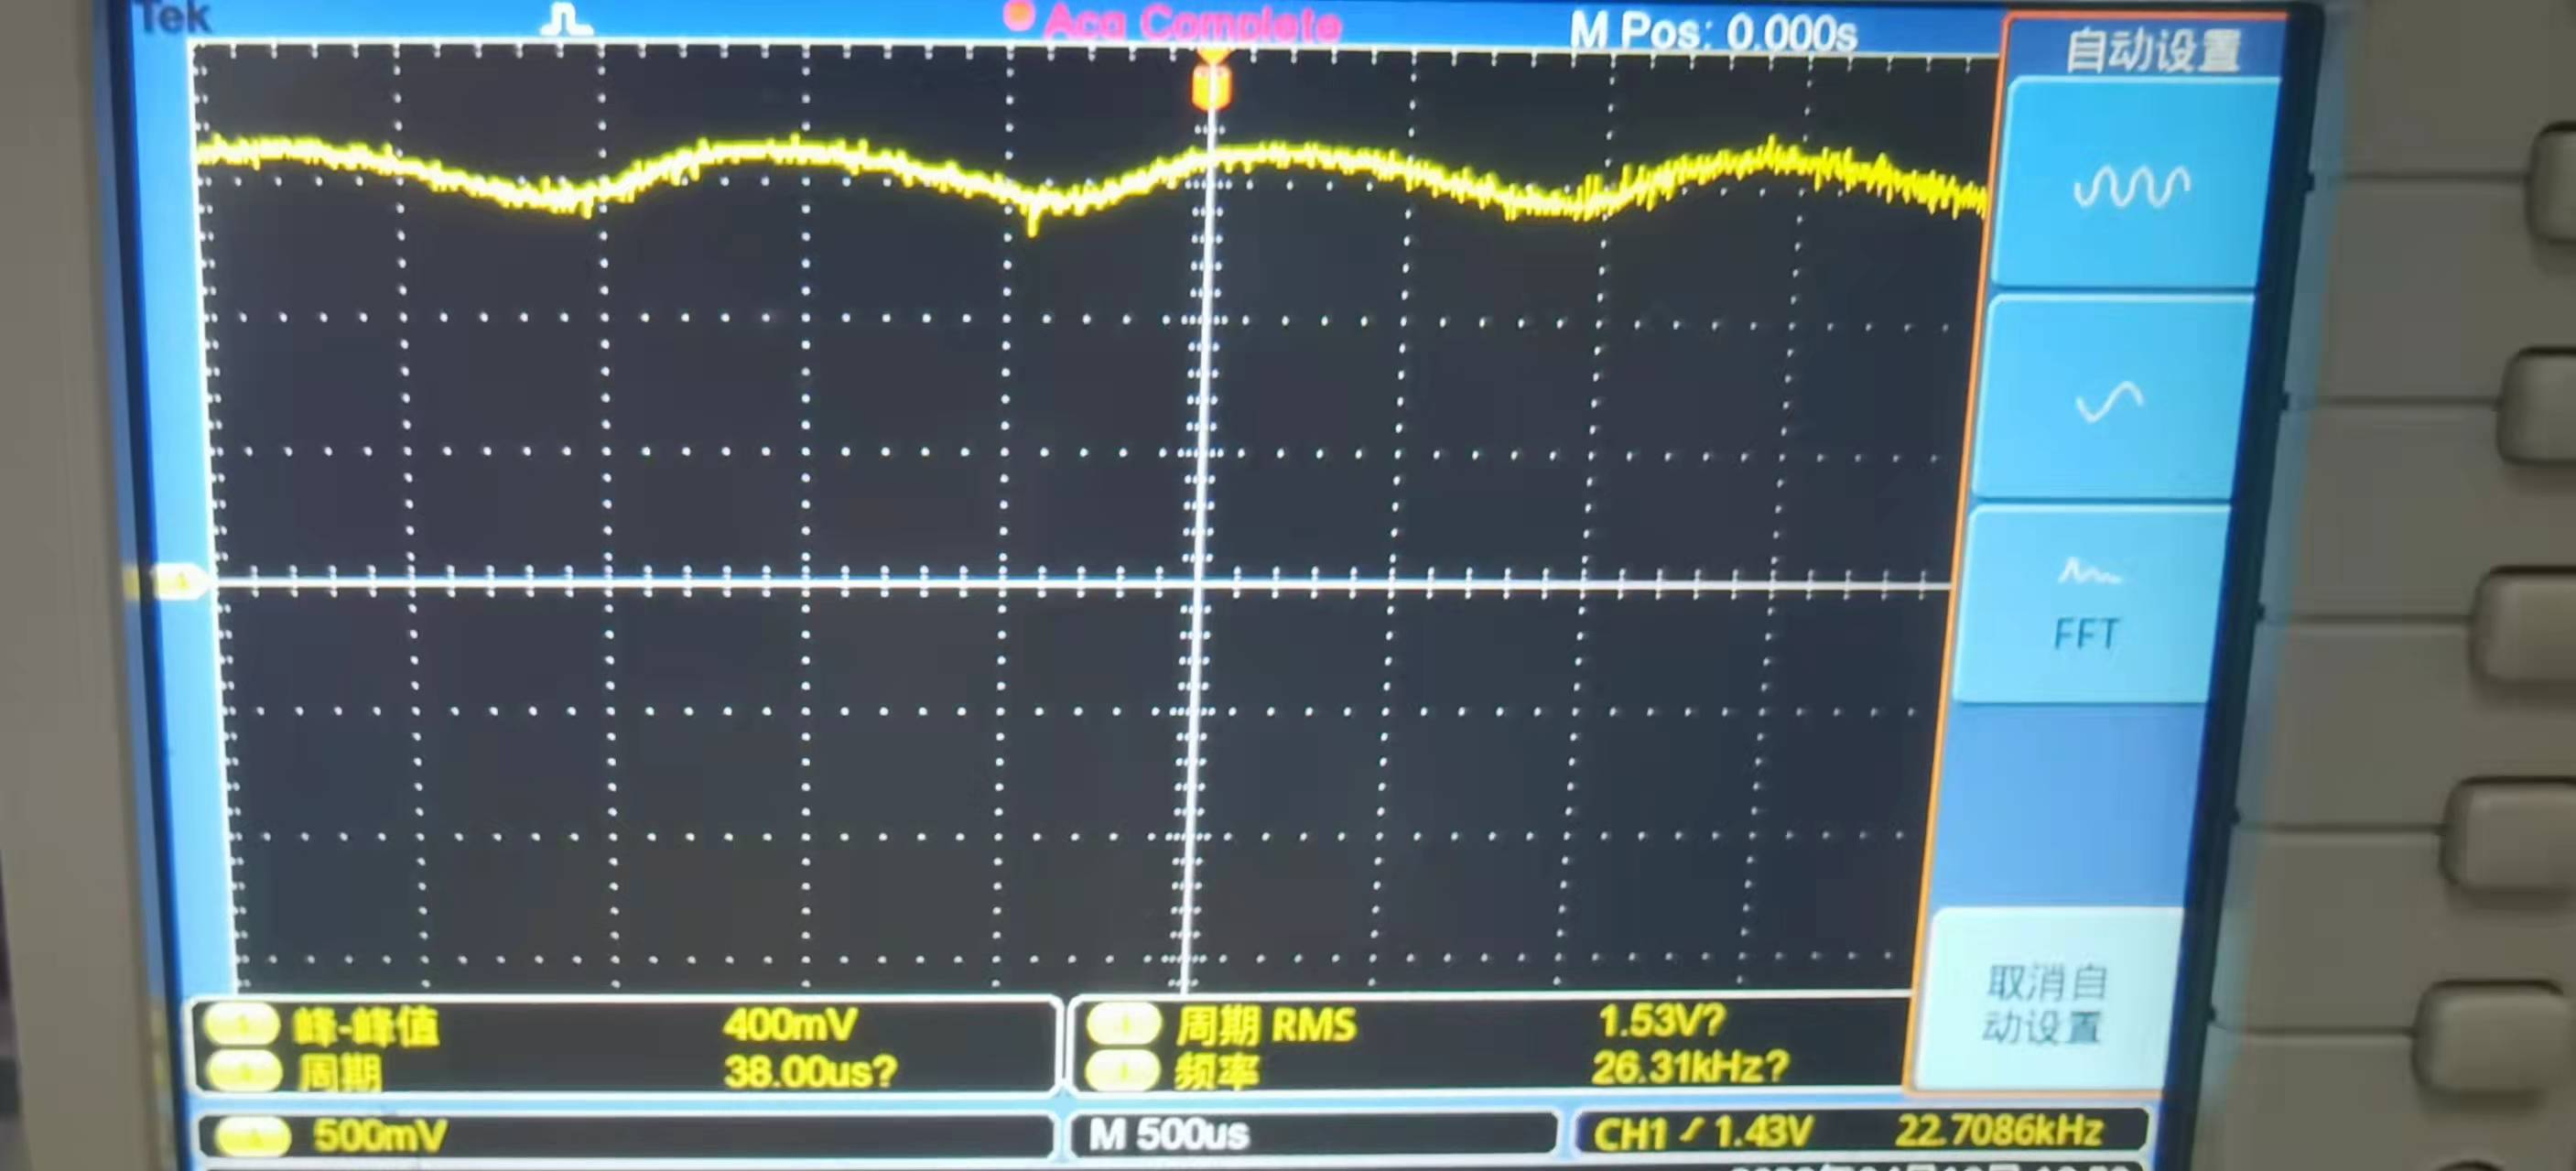
\includegraphics[width=0.7\linewidth]{img/original/10.jpg}
    \end{Figure}

    $10\mu F$单电容滤波信号:
    \begin{Figure}
        \centering
        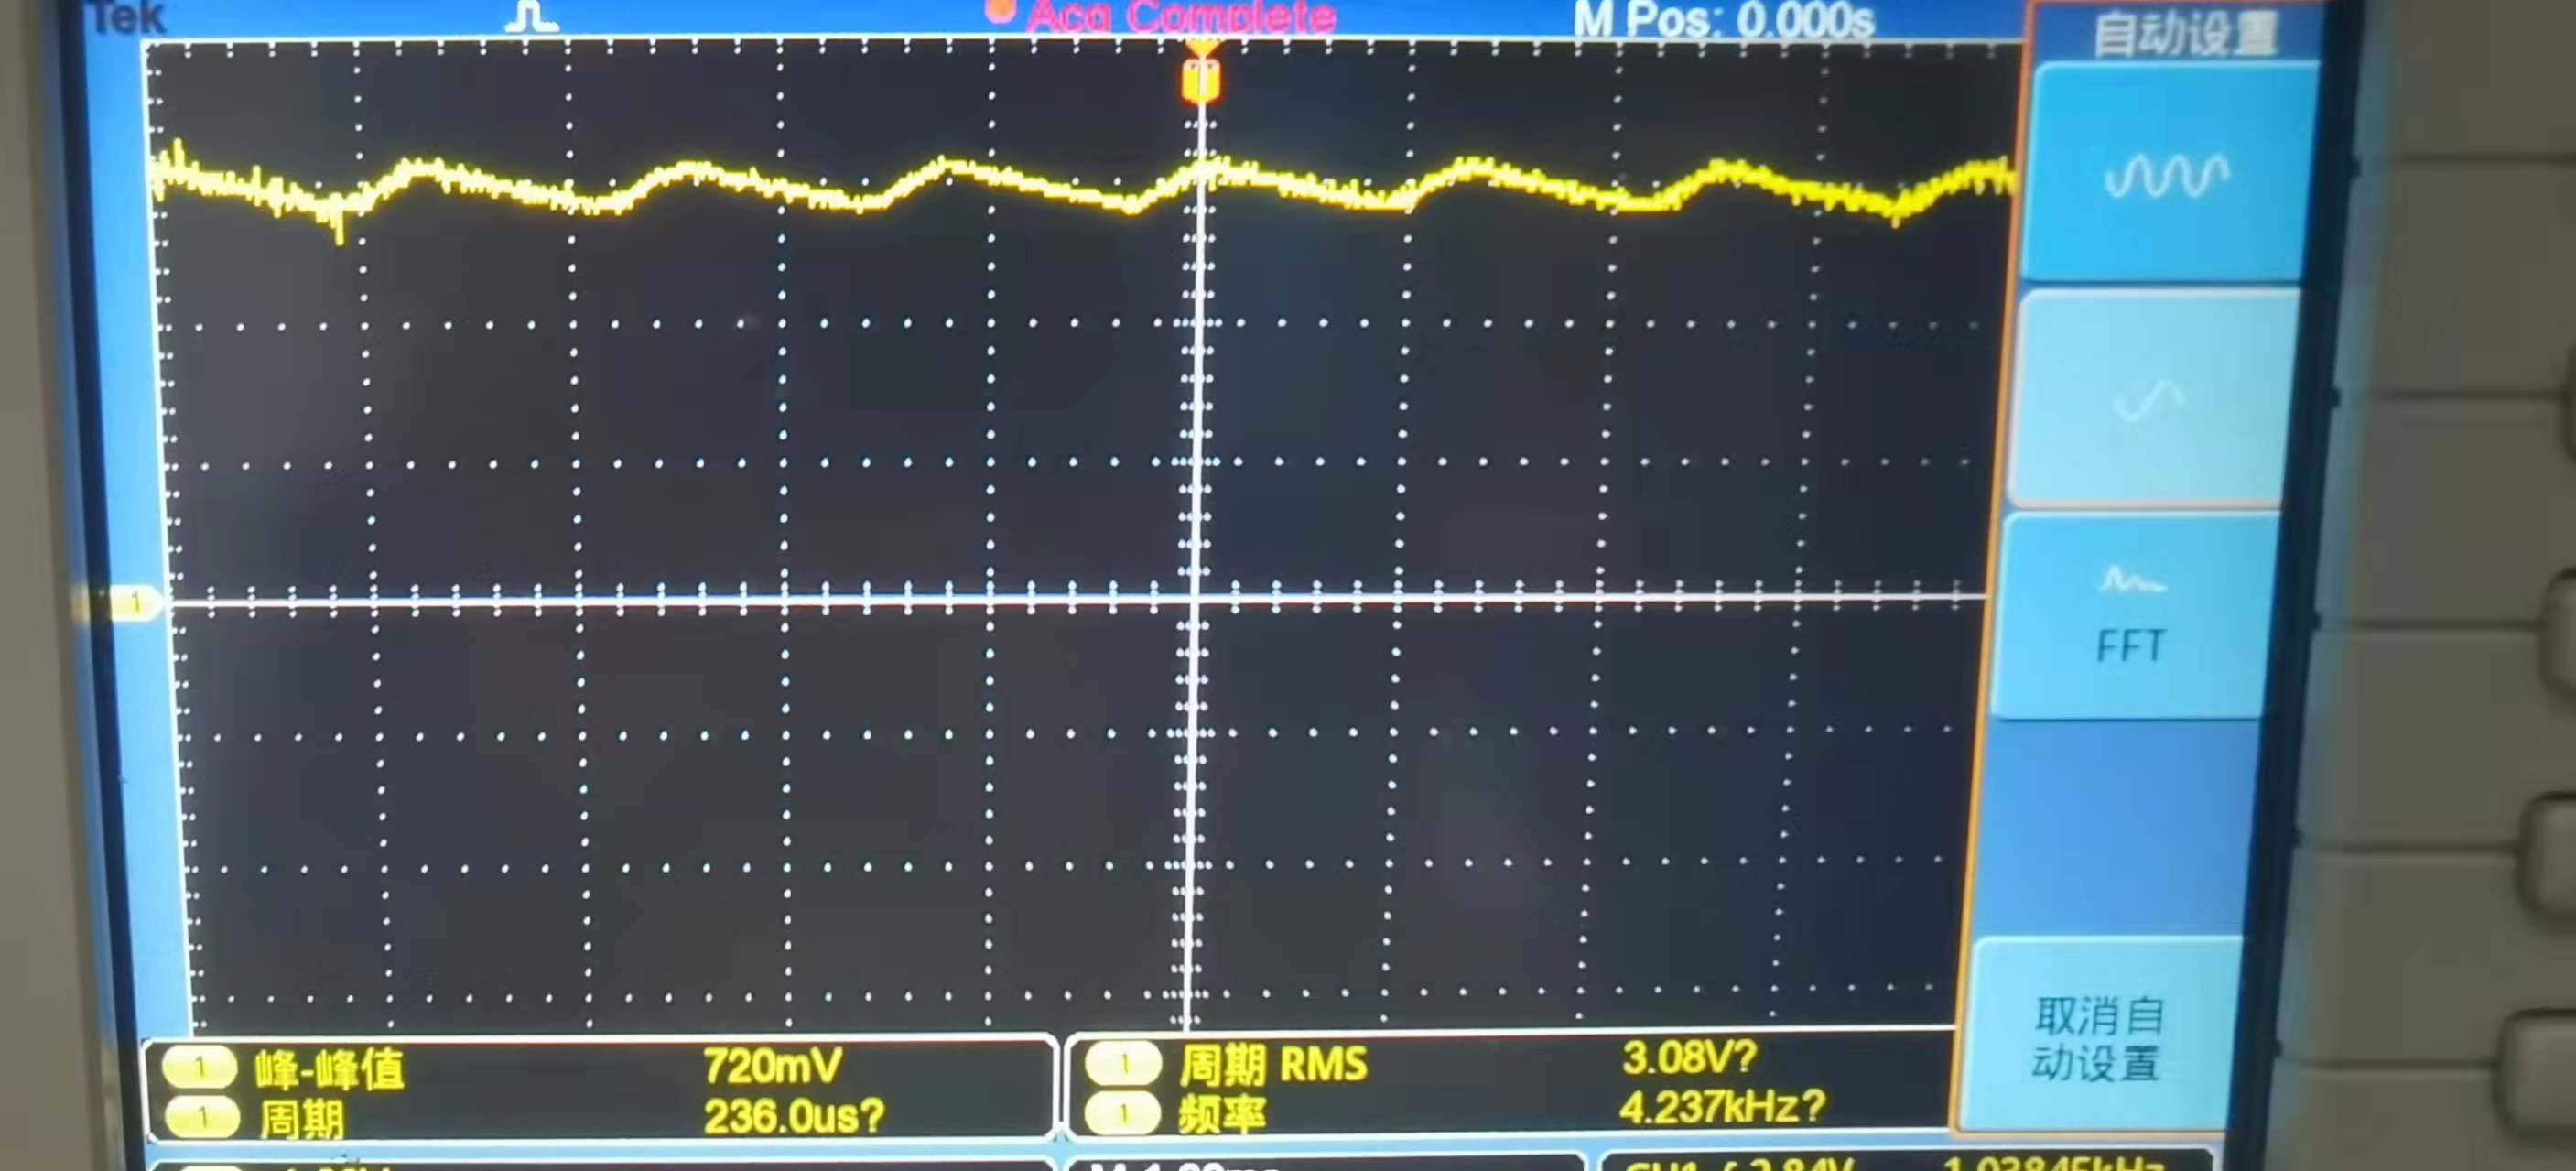
\includegraphics[width=0.7\linewidth]{img/original/7.jpg}
    \end{Figure}

    $10\mu F$ $\pi - RC$滤波信号:
    \begin{Figure}
        \centering
        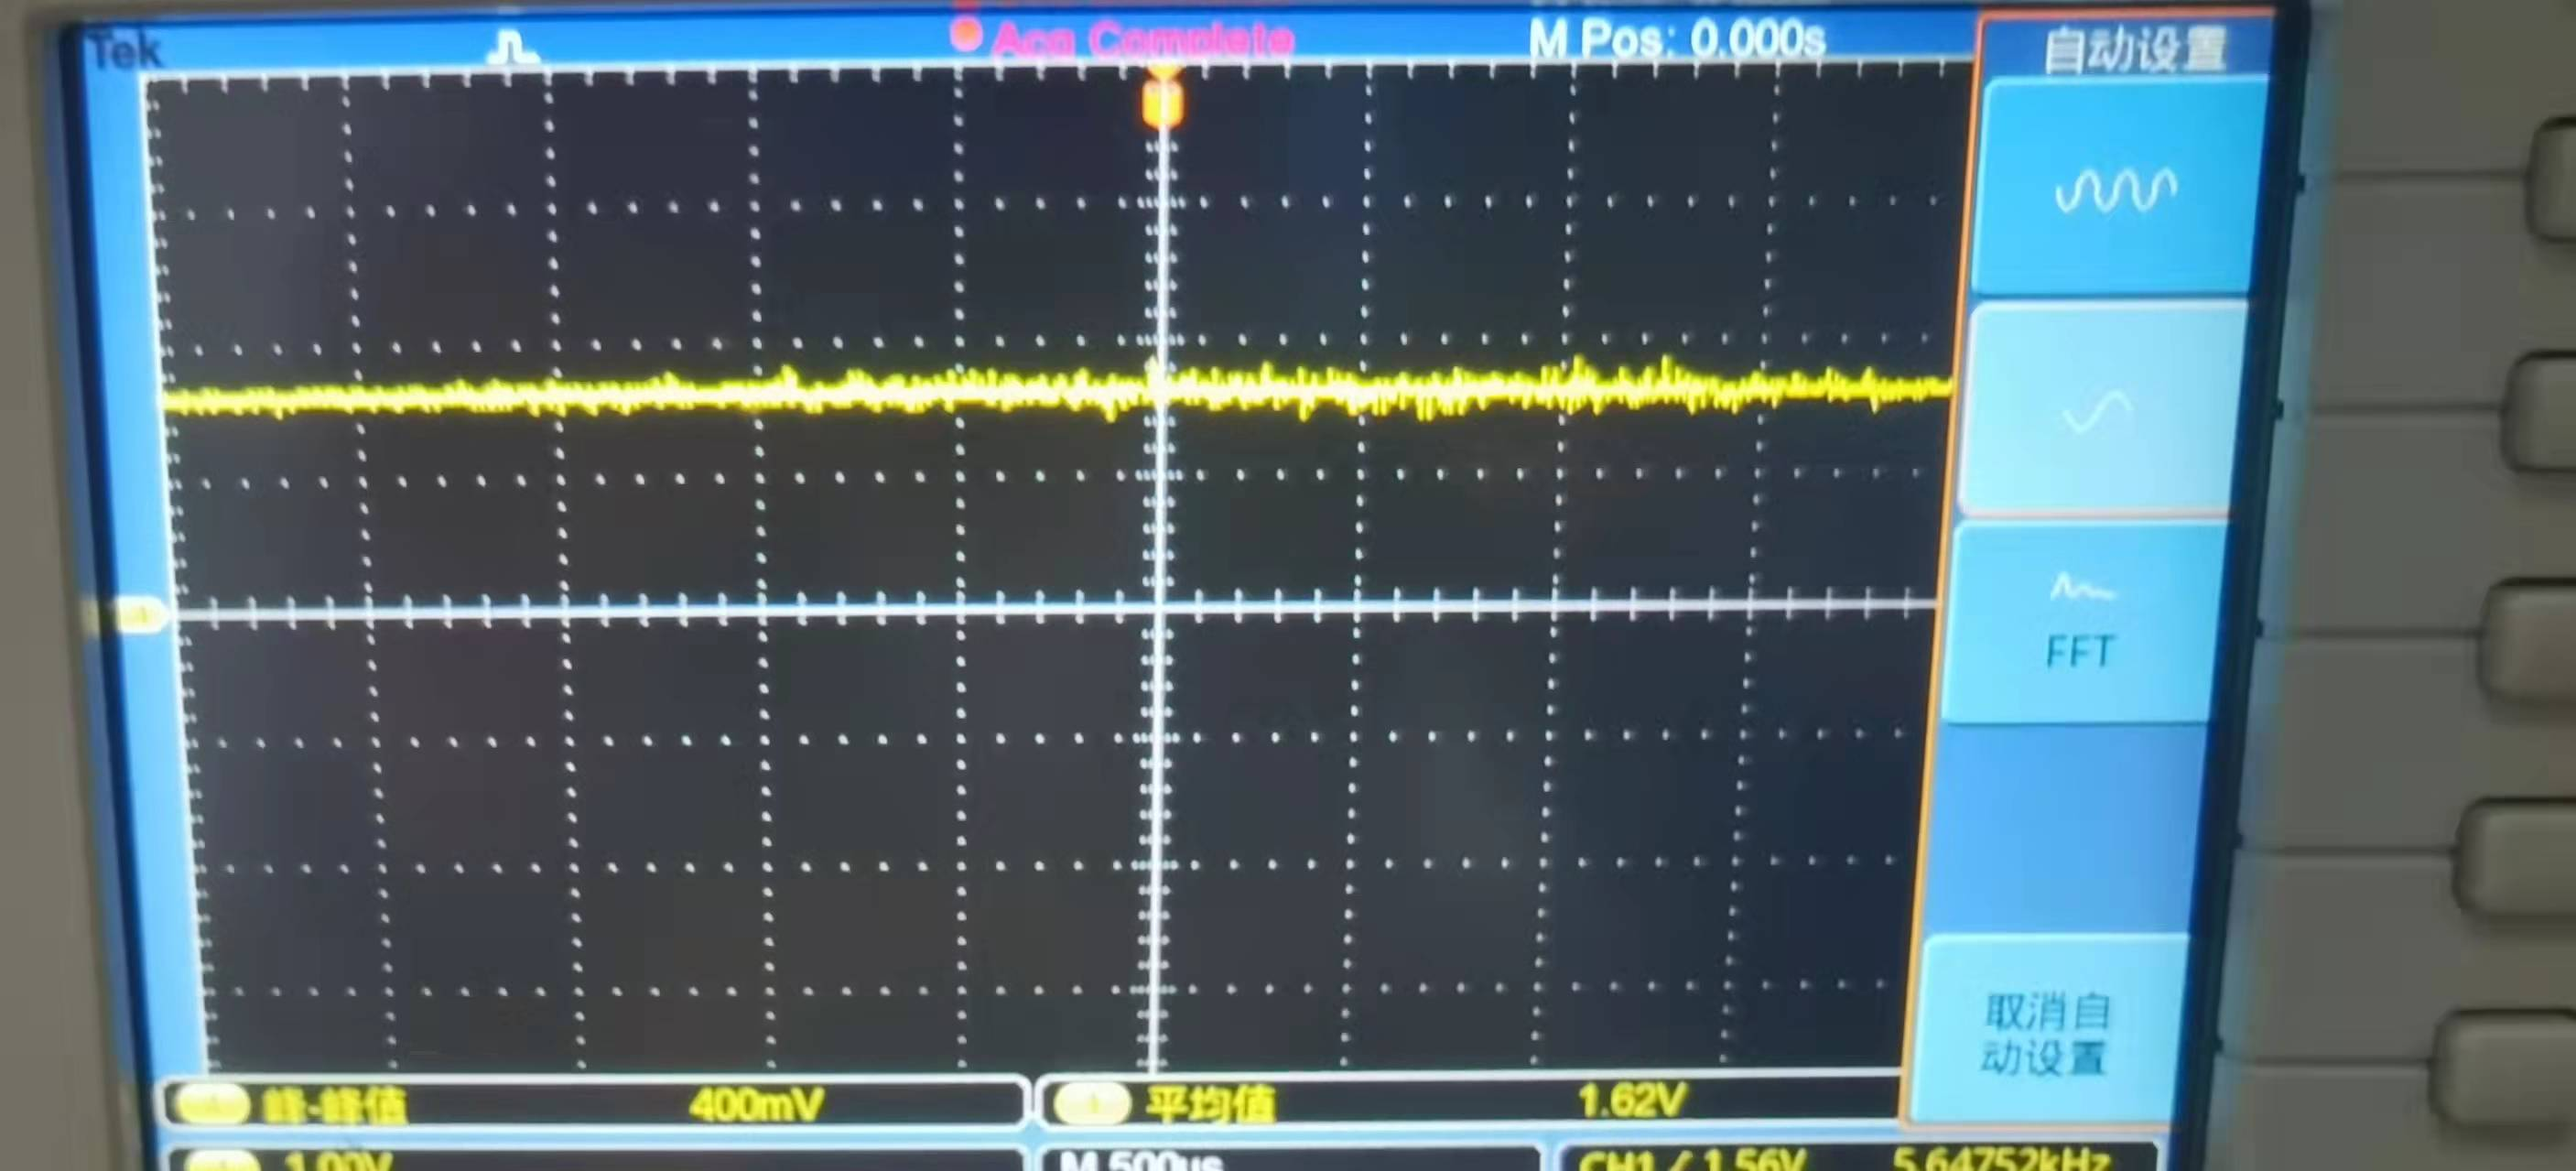
\includegraphics[width=0.7\linewidth]{img/original/6.jpg}
    \end{Figure}
\end{multicols}
\end{document}